%%% Hlavní soubor. Zde se definují základní parametry a odkazuje se na ostatní části. %%%

%% Verze pro jednostranný tisk:
% Okraje: levý 40mm, pravý 25mm, horní a dolní 25mm
% (ale pozor, LaTeX si sám přidává 1in)
\documentclass[12pt,a4paper]{report}
\setlength\textwidth{145mm}
\setlength\textheight{247mm}
\setlength\oddsidemargin{15mm}
\setlength\evensidemargin{15mm}
\setlength\topmargin{0mm}
\setlength\headsep{0mm}
\setlength\headheight{0mm}
% \openright zařídí, aby následující text začínal na pravé straně knihy
\let\openright=\clearpage

%% Pokud tiskneme oboustranně:
% \documentclass[12pt,a4paper,twoside,openright]{report}
% \setlength\textwidth{145mm}
% \setlength\textheight{247mm}
% \setlength\oddsidemargin{14.2mm}
% \setlength\evensidemargin{0mm}
% \setlength\topmargin{0mm}
% \setlength\headsep{0mm}
% \setlength\headheight{0mm}
% \let\openright=\cleardoublepage

%% Vytváříme PDF/A-2u
\usepackage[a-2u]{pdfx}

%% Přepneme na českou sazbu 
\usepackage[czech]{babel}
\usepackage[T1]{fontenc}
\usepackage{textcomp}

%% Použité kódování znaků: obvykle latin2, cp1250 nebo utf8:
\usepackage[utf8]{inputenc}

%%% Další užitečné balíčky (jsou součástí běžných distribucí LaTeXu)
\usepackage{amsmath}        % rozšíření pro sazbu matematiky
\usepackage{amsfonts}       % matematické fonty
\usepackage{amsthm}         % sazba vět, definic apod.
\usepackage{bbding}         % balíček s nejrůznějšími symboly
			    % (čtverečky, hvězdičky, tužtičky, nůžtičky, ...)
\usepackage{bm}             % tučné symboly (příkaz \bm)
\usepackage{graphicx}       % vkládání obrázků
\usepackage{fancyvrb}       % vylepšené prostředí pro strojové písmo
\usepackage{indentfirst}    % zavede odsazení 1. odstavce kapitoly
\usepackage[nottoc]{tocbibind} % zajistí přidání seznamu literatury,
                            % obrázků a tabulek do obsahu
\usepackage{icomma}         % inteligetní čárka v matematickém módu
\usepackage{dcolumn}        % lepší zarovnání sloupců v tabulkách
\usepackage{booktabs}       % lepší vodorovné linky v tabulkách
\usepackage{paralist}       % lepší enumerate a itemize
\usepackage{xcolor}         % barevná sazba

%% Změna písem na Libertine/Biolinum
\usepackage{libertinus}
\usepackage[libertine]{newtxmath}	%% Libertine v matematickém módu
\usepackage{inconsolata}

%% Úprava sazby pro lepší optický kerning a méně zalomených řádků
\usepackage{microtype}	

%%% Údaje o práci

% Název práce v jazyce práce (přesně podle zadání)
\def\NazevPrace{STP řešič pro OpenSMT}

% Název práce v angličtině
\def\NazevPraceEN{STP solver for OpenSMT}

% Jméno autora
\def\AutorPrace{Václav Luňák}

% Rok odevzdání
\def\RokOdevzdani{2020}

% Název katedry nebo ústavu, kde byla práce oficiálně zadána
% (dle Organizační struktury MFF UK, případně plný název pracoviště mimo MFF)
\def\Katedra{Katedra distribuovaných a~spolehlivých systémů}
\def\KatedraEN{Department of distributed and dependable systems}

% Jedná se o katedru (department) nebo o ústav (institute)?
\def\TypPracoviste{Katedra}
\def\TypPracovisteEN{Department}

% Vedoucí práce: Jméno a příjmení s~tituly
\def\Vedouci{doc.~RNDr.~Jan Kofroň,~Ph.D.}

% Pracoviště vedoucího (opět dle Organizační struktury MFF)
\def\KatedraVedouciho{Katedra distribuovaných a~spolehlivých systémů}
\def\KatedraVedoucihoEN{Department of distributed and dependable systems}

% Studijní program a obor
\def\StudijniProgram{Informatika}
\def\StudijniObor{Obecná informatika}

% Nepovinné poděkování (vedoucímu práce, konzultantovi, tomu, kdo
% zapůjčil software, literaturu apod.)
\def\Podekovani{%
Poděkování.
}

% Abstrakt (doporučený rozsah cca 80-200 slov; nejedná se o zadání práce)
\def\Abstrakt{%
Abstrakt.
}
\def\AbstraktEN{%
Abstract.
}

% 3 až 5 klíčových slov (doporučeno), každé uzavřeno ve složených závorkách
\def\KlicovaSlova{%
{klíčová} {slova}
}
\def\KlicovaSlovaEN{%
{key} {words}
}

%% Balíček hyperref, kterým jdou vyrábět klikací odkazy v PDF,
%% ale hlavně ho používáme k uložení metadat do PDF (včetně obsahu).
%% Většinu nastavítek přednastaví balíček pdfx.
\hypersetup{unicode}
\hypersetup{breaklinks=true}

%% Definice různých užitečných maker (viz popis uvnitř souboru)
%%% Tento soubor obsahuje definice různých užitečných maker a prostředí %%%
%%% Další makra připisujte sem, ať nepřekáží v ostatních souborech.     %%%

%%% Drobné úpravy stylu

% Tato makra přesvědčují mírně ošklivým trikem LaTeX, aby hlavičky kapitol
% sázel příčetněji a nevynechával nad nimi spoustu místa. Směle ignorujte.
\makeatletter
\def\@makechapterhead#1{
  {\parindent \z@ \raggedright \normalfont
   \Huge\bfseries \thechapter. #1
   \par\nobreak
   \vskip 20\p@
}}
\def\@makeschapterhead#1{
  {\parindent \z@ \raggedright \normalfont
   \Huge\bfseries #1
   \par\nobreak
   \vskip 20\p@
}}
\makeatother

% Toto makro definuje kapitolu, která není očíslovaná, ale je uvedena v obsahu.
\def\chapwithtoc#1{
\chapter*{#1}
\addcontentsline{toc}{chapter}{#1}
}

% Trochu volnější nastavení dělení slov, než je default.
\lefthyphenmin=2
\righthyphenmin=2

% Zapne černé "slimáky" na koncích řádků, které přetekly, abychom si
% jich lépe všimli.
\overfullrule=1mm

%%% Makra pro definice, věty, tvrzení, příklady, ... (vyžaduje baliček amsthm)

\theoremstyle{plain}
\newtheorem{veta}{Věta}
\newtheorem{lemma}[veta]{Lemma}
\newtheorem{tvrz}[veta]{Tvrzení}

\theoremstyle{plain}
\newtheorem{definice}{Definice}

\theoremstyle{remark}
\newtheorem*{dusl}{Důsledek}
\newtheorem*{pozn}{Poznámka}
\newtheorem*{prikl}{Příklad}

%%% Prostředí pro důkazy

\newenvironment{dukaz}{
  \par\medskip\noindent
  \textit{Důkaz}.
}{
\newline
\rightline{$\qedsymbol$}
}

%%% Prostředí pro sazbu kódu, případně vstupu/výstupu počítačových
%%% programů. (Vyžaduje balíček fancyvrb -- fancy verbatim.)

\DefineVerbatimEnvironment{code}{Verbatim}{fontsize=\small, frame=single}

%%% Prostor reálných, resp. přirozených čísel
\newcommand{\R}{\mathbb{R}}
\newcommand{\N}{\mathbb{N}}

%%% Užitečné operátory pro statistiku a pravděpodobnost
\DeclareMathOperator{\pr}{\textsf{P}}
\DeclareMathOperator{\E}{\textsf{E}\,}
\DeclareMathOperator{\var}{\textrm{var}}
\DeclareMathOperator{\sd}{\textrm{sd}}

%%% Příkaz pro transpozici vektoru/matice
\newcommand{\T}[1]{#1^\top}

%%% Vychytávky pro matematiku
\newcommand{\goto}{\rightarrow}
\newcommand{\gotop}{\stackrel{P}{\longrightarrow}}
\newcommand{\maon}[1]{o(n^{#1})}
\newcommand{\abs}[1]{\left|{#1}\right|}
\newcommand{\dint}{\int_0^\tau\!\!\int_0^\tau}
\newcommand{\isqr}[1]{\frac{1}{\sqrt{#1}}}

%%% Vychytávky pro tabulky
\newcommand{\pulrad}[1]{\raisebox{1.5ex}[0pt]{#1}}
\newcommand{\mc}[1]{\multicolumn{1}{c}{#1}}

%%% Moje makra
\newcommand{\Solver}{\emph{Solver\textsubscript{T}} }
\newcommand{\icode}{\texttt}
\newcommand{\Z}{\mathbb{Z}}


%% Titulní strana a různé povinné informační strany
\begin{document}
%%% Titulní strana práce a další povinné informační strany

%%% Titulní strana práce

\pagestyle{empty}
\hypersetup{pageanchor=false}

\begin{center}

\centerline{\mbox{
\includegraphics[width=166mm]{./img/logo-cs.pdf}}}

\vspace{-8mm}
\vfill

{\bf\Large BAKALÁŘSKÁ PRÁCE}

\vfill

{\LARGE\AutorPrace}

\vspace{15mm}

{\LARGE\bfseries\NazevPrace}

\vfill

\Katedra

\vfill

{
\centerline{\vbox{\halign{\hbox to 0.45\hsize{\hfil #}&\hskip 0.5em\parbox[t]{0.45\hsize}{\raggedright #}\cr
Vedoucí bakalářské práce:&\Vedouci \cr
\noalign{\vspace{2mm}}
Studijní program:&\StudijniProgram \cr
\noalign{\vspace{2mm}}
Studijní obor:&\StudijniObor \cr
}}}}

\vfill

% Zde doplňte rok
Praha \RokOdevzdani

\end{center}

\newpage

%%% Následuje vevázaný list -- kopie podepsaného "Zadání bakalářské práce".
%%% Toto zadání NENÍ součástí elektronické verze práce, nescanovat.

%%% Strana s čestným prohlášením k bakalářské práci

\openright
\hypersetup{pageanchor=true}
\pagestyle{plain}
\pagenumbering{roman}
\vglue 0pt plus 1fill

\noindent
Prohlašuji, že jsem tuto bakalářskou práci vypracoval(a) samostatně a~výhradně
s~použitím citovaných pramenů, literatury a~dalších odborných zdrojů.
Tato práce nebyla využita k získání jiného nebo stejného titulu.

\medskip\noindent
Beru na~vědomí, že se na moji práci vztahují práva a~povinnosti vyplývající
ze zákona č. 121/2000 Sb., autorského zákona v~platném znění, zejména skutečnost,
že Univerzita Karlova má právo na~uzavření licenční smlouvy o~užití této
práce jako školního díla podle §60 odst. 1 autorského zákona.

\vspace{10mm}

\hbox{\hbox to 0.5\hsize{%
V \hbox to 6em{\dotfill} dne \hbox to 6em{\dotfill}
\hss}\hbox to 0.5\hsize{\dotfill\quad}}
\smallskip
\hbox{\hbox to 0.5\hsize{}\hbox to 0.5\hsize{\hfil Podpis autora\hfil}}

\vspace{20mm}
\newpage

%%% Poděkování

\openright

\noindent
\Podekovani

\newpage

%%% Povinná informační strana bakalářské práce

\openright

\vbox to 0.5\vsize{
\setlength\parindent{0mm}
\setlength\parskip{5mm}

Název práce:
\NazevPrace

Autor:
\AutorPrace

\TypPracoviste:
\Katedra

Vedoucí bakalářské práce:
\Vedouci, \KatedraVedouciho

Abstrakt:
\Abstrakt

Klíčová slova:
\KlicovaSlova

\vss}\nobreak\vbox to 0.49\vsize{
\setlength\parindent{0mm}
\setlength\parskip{5mm}

Title:
\NazevPraceEN

Author:
\AutorPrace

\TypPracovisteEN:
\KatedraEN

Supervisor:
\Vedouci, \KatedraVedoucihoEN

Abstract:
\AbstraktEN

Keywords:
\KlicovaSlovaEN

\vss}

\newpage

\openright
\pagestyle{plain}
\pagenumbering{arabic}
\setcounter{page}{1}


%%% Strana s automaticky generovaným obsahem bakalářské práce

\tableofcontents

%%% Jednotlivé kapitoly práce jsou pro přehlednost uloženy v samostatných souborech
\chapter*{Úvod}
\addcontentsline{toc}{chapter}{Úvod}

V~mnoha informatických oblastech se setkáváme s~potřebou vyjádřit nějakou časovou informaci. Ať už se pohybujeme na poli plánování, formální verifikace nebo paralelního programování, mohou se na naši práci vztahovat časová omezení, na která musíme brát zřetel. Není tedy divu, že s~postupným vývojem těchto disciplín roste potřeba pro efektivní způsoby, kterými bychom tato omezení mohli analyzovat.

Jedním z~nejzákladnějších a~nejběžnějších typů časových omezení jsou takzvaná \emph{rozdílová omezení}. Jak už napovídá jejich název, týkají se časového rozdílu mezi dvěma událostmi. Matematickým formalizmem bychom mohli rozdílové omezení definovat například ve tvaru $X_i - X_j \in [t_1, t_2]$ nebo ekvivalentně jako $X_i - X_j \leq t$. Vzhledem k~relativní jednoduchosti takové podmínky byl problém splnitelnosti konjunkce rozdílových omezení nazván \emph{simple temporal problem} (STP). Přes jejich zdánlivou přímočarost se ale rozdílová omezení ukázala jako dostatečně expresivní pro velkou řadu problémů. Uvažujme například následující situaci, jejíž paralely můžeme nalézt v~oblasti plánování: 

\begin{center}
\begin{minipage}{\textwidth}
Na strojích $s_1 \dots s_n$ potřebujeme provést celkem $m$ úkolů. Každý úkol se skládá z~nějakého množství operací. Každá operace musí proběhnout na konkrétním stroji a~zabere nějaký čas. Operace náležící témuž úkolu navíc musí proběhnout v~pevně daném pořadí. Dokážeme jednotlivé operace rozplánovat mezi všechny stroje tak, aby výpočet skončil před cílovým časem $T$?
\end{minipage}
\end{center}

Příklad převodu takového zadání do tvaru rozdílových omezení ukazuje obrázek \ref{fig:job}. První druh nerovnic zajišťuje smysluplný počátek pro všechny operace. Nerovnice druhého typu určují následnost operací v~jednotlivých úkolech a podmínky třetího typu označují fakt, že na jednom stroji může v~jednu chvíli probíhat nejvýše jedna operace. Chceme-li navíc operace dokončit před časem $T$, musíme je začít s dostatečným předstihem, což vyjadřuje poslední druh nerovnic. 

Jistě není těžké představit si reálná využití pro řešení takového problému. Jak si ale můžeme všimnout, už se nejedná o~běžný STP --- v~problému se navíc objevují disjunkce omezení. Naše podmínky obecně odpovídají výrokové formuli (v~konjunktivní normální formě), jejíž atomy jsou rozdílová omezení. Problém splnitelnosti takovýchto formulí se obecně nazývá \emph{satisfiability modulo theories} (SMT) a~je důležitým předmětem zkoumání v~oboru formální verifikace~\cite{SMT}. Přestože je tento problém obecně složitější než STP, ukážeme si, že jeho rozhodnutí jsme stále schopni dosáhnout vhodným využitím postupů na řešení STP.

\begin{figure}[b]
	\centering
	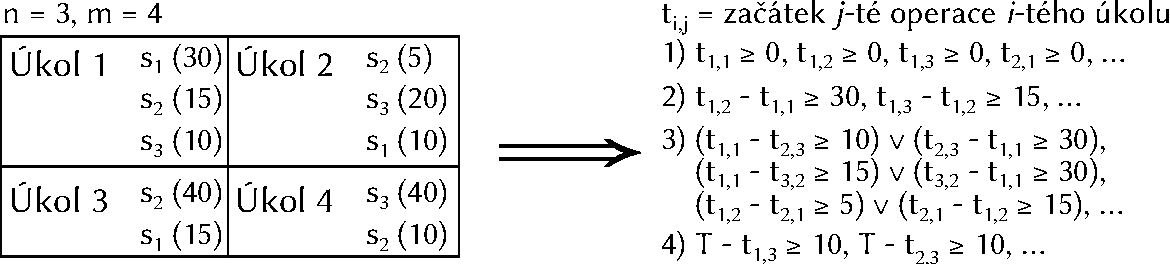
\includegraphics[width=\textwidth]{jobshop.pdf}
	\caption{Příklad převodu plánovacího problému do rozdílových omezení} 
	\label{fig:job}
\end{figure}
\newpage
Cílem této práce je vytvoření STP řešiče pro SMT řešič OpenSMT~\cite{OpenSMT}. Nejprve si přiblížíme některé základní principy z~oblasti SMT řešičů. Následně analyzujeme existující postupy pro řešení STP v~kontextu SMT a~navrhneme podle nich konkrétní algoritmus pro zapojení do OpenSMT. Navržený algoritmus následně implementujeme. Jako součást práce také naši implementaci otestujeme na rozsáhlé sadě problémů a~srovnáme její účinnost s~existujícími SMT řešiči.

\chapter{Analýza}

\section{Prostředí}

Požadavky na použité prostředí jsou určeny převážně požadavky frameworku OpenSMT, pod nějž tato práce spadá. OpenSMT --- a~tudíž i~tento projekt --- je programován v~jazyce C++, konkrétně ve verzi C++11. Práce byla vyvíjena a~testována na operačním systému s~linuxovým jádrem nad architekturou x64. Jelikož si nejsme vědomi toho, že bychom použili vlastnosti jazyka specifické pro tuto konfiguraci, věříme, že náš kód bude možné bez větších potíží zprovoznit i~na jiných platformách a~operačních systémech.

\section{Fungování SMT řešičů}\label{smt}

Vzhledem k~podobnostem mezi SAT a~SMT není překvapením, že SMT řešiče využívají schopností SAT řešičů. Přechod mezi rozhraním termů teorie a~SAT řešičem zpravidla probíhá jedním ze dvou základních způsobů \cite{Nieuwenhuis05}.

První přístup se nazývá \emph{hladový}. Hladové SMT řešiče operují ve dvou krocích. V~prvním převedou celou vstupní formuli na ekvisplnitelnou booleovskou formuli. Druhý krok pak již spočívá jen v~předání této formule existujícímu SAT řešiči. Pokud bychom tedy pracovali například s~aritmetikou nad osmibitovými čísly, mohli bychom reprezentovat každou proměnnou osmi binárními proměnnými a~aritmetické operace převézt na odpovídající sekvence logických operací.

Nespornou výhodou hladových řešičů je možnost použití již existujících metod implementovaných na řešení SAT. Pro některé teorie se také hladové řešiče ukazují být rychlejší než jejich alternativy. Jejich největší problém pak obecně spočívá v~překladu literálů teorie do booleovských formulí. Ten musí být zkonstruován samostatně pro každou teorii, a~navíc může v~závislosti na teorii produkovat formule výrazně (často exponenciálně) delší, než byl původní vstup. Efektivní převody existují např. pro EUF s~omezenou doménou \cite{randal02}, obecně však hladový přístup není příliš rozšířený.

Jeho protějškem je takzvaný \emph{líný přístup}. Líný přístup se nesnaží měnit strukturu vstupní formule; namísto toho je každý predikát abstrahován pomocí nové binární proměnné. Když pak SAT řešič rozhodne o~ohodnocení těchto proměnných, oznámí toto rozhodnutí dedikovanému \emph{řešiči teorie}\footnote{Použitím pojmu \emph{řešič} bez přívlastku rozumíme v~této práci právě řešič teorie.}. Řešič teorie je schopen určit, zda je dané ohodnocení konzistentní, tzn.~dokáže rozhodnout o~splnitelnosti nějaké konjunkce literálů této teorie. SAT řešič potom hledá platná ohodnocení, dokud nenajde takové, které řešič teorie prohlásí za konzistentní.

Ve prospěch líných SMT řešičů svědčí fakt, že pro danou teorii často existují dobře známé postupy na ověření konjunkce literálů. Pro LA například můžeme využít metod lineárního programování, řešič teorie DL řeší STP (viz.~\ref{stp}) a~podobně. Líné řešiče však mohou ztrácet efektivitu zejména v~důsledku \emph{slepého prohledávání} \cite{Moura04}, kde hlavní řešič rozhoduje o~hodnotě predikátů, aniž by a~priori věděl o~důsledcích těchto ohodnocení v~rámci teorie, což může vést k~nutnosti vyzkoušet velké množství ohodnocení, než je nalezeno nějaké, které je s~teorií konzistentní.

V~roce 2004 navrhli Gazinger a~kol. nový přístup zvaný \emph{DPLL(T)} \cite{Gazinger04}. DPLL($T$) má koncepčně blíže k~línému vyhodnocování, integruje však těsněji hlavní řešič s~řešiči teorie. Místo toho, aby využíval řešiče teorie až po nalezení nějakého ohodnocení, průběžně mu oznamuje dosavadní rozhodnutí a~periodicky se ho ptá na splnitelnost právě dosazené konjunkce. Řešič teorie pak kromě kontroly splnitelnosti také oznamuje hlavnímu řešiči důsledky této konjunkce. Tím jsme schopni dříve opustit větve rozhodovacího stromu nekonzistentní s~teorií. 

V~jádru tohoto přístupu stojí obecný DPLL($X$) engine, využívající DPLL \cite{Davis60} postupu pro SAT řešiče. Tento engine nemusí mít žádné znalosti o~konkrétní teorii. Dosazením řešiče \Solver dané teorie $T$ za parametr $X$ pak vytvoříme konkrétní instanci DPLL($T$). Hlavní engine přitom v~průběhu výpočtu komunikuje se \Solver.

Stejně jako u~líných řešičů, v~DPLL($T$) abstrahuje \Solver literály teorie za běžné booleovské proměnné, se kterými může DPLL($X$) pracovat. Než tedy začne samotný výpočet, musí být \Solver poskytnuta vstupní formule, aby bylo možné provést tuto transformaci. Jakmile pak engine během výpočtu rozhodne o~pravdivostní hodnotě některého abstrahovaného literálu, okamžitě toto rozhodnutí oznámí řešiči teorie. Ten musí rozhodnout, zda je ohodnocení konzistentní s~předešlými ohodnocenými literály. Může navíc objevit nějaké důsledky tohoto ohodnocení v~teorii. Výsledek \Solver předá zpět DPLL($X$), který podle něj určí další postup. 

Pokud se ukáže ohodnocení jako konzistentní, pokračuje v~rozhodování o~pravdivosti dalších literálů. Bere přitom ohled na nalezené důsledky. Je-li naopak ohodnocení sporné, musí analyzovat příčinu sporu a~vrátit se zpět do stavu, kdy byl ještě konzistentní. \Solver musí být pro tento případ schopen předávat informace vysvětlující jeho rozhodnutí, poněvadž jako jediný zná vztahy mezi abstrahovanými proměnnými. Samozřejmě se pak od něj vyžaduje také schopnost vrátit se do předchozího stavu, tj.~zapomenout určitý počet nejpozději přidaných ohodnocení.

Vzhledem k~těmto požadavků na \Solver dospěli autoři frameworku~\cite{Gazinger04} k~následujícímu rozhranní propojujícím řešič teorie s~DPLL($X$):

\begin{description}
	\item[Initialize(L: množina literálů).] Inicializuje \Solver množinou literálů $L$, které se vyskytují v~problému.
	\item[SetTrue(l: L-literál): množina L-literálů.] Pokud se $l$ ukáže konzistentní s~předchozími ohodnoceními, přidá ho do seznamu zadaných literálů a~vrátí nějakou množinu důsledků tohoto přidání. V~opačném případě vyvolá výjimku vyjadřující spornost $l$ s~dosud zadanými literály. S~ohledem na výkonnost řešiče může být vrácená množina důsledků neúplná (popř. úplně prázdná).
	\item[IsTrue?(l: L-literál): boolean.] Vrátí \emph{true} právě tehdy, když $l$ je důsledkem seznamu přidaných literálů. Vrací \emph{false}, pokud je důsledkem tohoto seznamu $\neg l$, nebo pokud z~něj nevyplývá ani $l$, ani $\neg l$.
	\item[Backtrack(n: přir. číslo).] Odstraní posledních $n$ hodnot ze seznamu zadaných literálů. $n$ nesmí být větší než velikost tohoto seznamu.
	\item[Explain(l: L-literál): množina L-literálů.] Vrátí pokud možno co nejmenší podmnožinu zadaných literálů, z~jejichž konjunkce plyne $l$. Pro $l$ musí platit, že je důsledkem nějaké takové podmnožiny, tedy musí být obsažen v~návratové hodnotě nějakého volání \icode{SetTrue($l'$)} takového, že $l'$ nebylo zahozeno žádným následným voláním \icode{Backtrack}.
\end{description}

Při použití tohoto rozhranní přitom \Solver nemusí nic vědět o~implementaci DPLL($X$) enginu. Framework je tedy velice modulární a~snadno rozšiřitelný o~nové teorie. Vyžadujeme pouze, aby byl \Solver schopný inkrementálně přijímat a~odebírat jednotlivé literály teorie. Tento postup se v~praxi ukazuje jako efektivnější než dostupné alternativy. Většina dnes rozšířených SMT řešičů --- včetně námi používaného OpenSMT2 --- je tedy založena na metodě DPLL($T$).

\section{Převod STP na grafový problém}\label{graf}

Velkou rozšířenost STP můžeme mimo jiné přisoudit tomu, že jsme schopni ho efektivně řešit. Jelikož se problém skládá výlučně z~lineárních omezení, mohli bychom na první pohled využít metod lineárního programování, jako je například simplexový algoritmus. Tyto metody jsou schopny řešit i~mnohem komplexnější problémy, avšak s~jejich výpočetní silou se pojí znatelně vyšší časová náročnost. Algoritmy specializované na STP se proto už od svého počátku \cite[Kapitola 2]{Dechter91} obracejí jiným směrem, a~to k~formalizmu teorie grafů. Přestože v~průběhu let vzikly různé metody řešení tohoto problému, všechny fungují na základě převedení množiny omezení na takzvaný \emph{omezující graf}.

\begin{definice}[Omezující graf]
	Nechť $\Pi$ je množina rozdílových omezení. Omezujícím grafem této množiny rozumíme hranově ohodnocený orientovaný graf G takový, že vrcholy G tvoří proměnné vyskytující se v~$\Pi$ a~každému omezení $(x-y \leq c) \in \Pi$ odpovídá v~G hrana $\langle x,y\rangle$ s~ohodnocením $c$.
\end{definice}
\begin{pozn}
	Hranu $\langle x,y\rangle$ s~ohodnocením $c$ budeme značit $x \xrightarrow{c} y$. Orientovanou cestu z~$x$ do $y$ se součtem ohodnocení $k$ pak budeme značit $x \xrightarrow{k*} y$.
\end{pozn}

Pro úplnost dodejme, že dvojice proměnných se může vyskytovat v~libovolně mnoha omezeních. Omezující graf je tedy formálně orientovaným multigrafem. Vzhledem k~vzájemné bijekci mezi hranami grafu a~nerovnicemi problému budeme v~průběhu práce volně přecházet mezi oběma reprezentacemi.

\begin{figure}
	\centering
	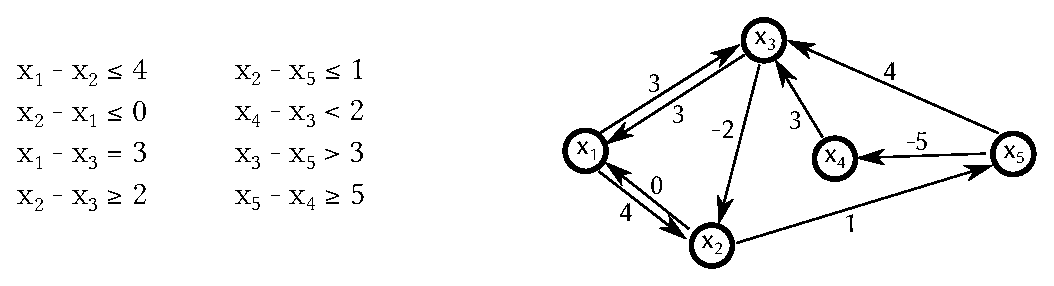
\includegraphics[width=\textwidth]{graph_example}
	\caption{Převod STP problému nad $\Z$ na omezující graf}
\end{figure}

Převod do formy grafu je pro řešení problému zásadní. Umožňuje nám totiž formulovat následující klíčové tvrzení.

\begin{tvrz}[Dechter a~kol. \cite{Dechter91}]
	Nechť $\Pi$ je množina rozdílových omezení. Instance STP tvořená touto množinou je splnitelná právě tehdy, když omezující graf $\Pi$ neobsahuje záporné cykly.
\end{tvrz}
\begin{proof}
	Najdeme-li v~omezujícím grafu záporný cyklus obsahující vrchol $x$, sečtením všech nerovnic vyskytujících se v~tomto cyklu dostaneme $x-x \leq c < 0$, z~čehož je jasně problém nesplnitelný. Je-li na druhou stranu problém nesplnitelný, obsahuje $\Pi$ nějakou nerovnici $x - y \leq c$ takovou, že z~$\Pi$ vyplývá $y - x < -c$. Tato implikace znamená, že v~omezujícím grafu existuje cesta $y \xrightarrow{k*} x$ taková, že $k < -c$. Hrana $x \xrightarrow{c} y$ pak společně s~touto cestou tvoří záporný cyklus.
\end{proof}

Hledání splnitelnosti STP jsme tedy schopni převést na hledání záporného cyklu v~grafu. To je problém, který dokážeme efektivně řešit. Využít můžeme např. některý algoritmus na hledání nejkratší cesty, kupříkladu Floydův-Warshallův algoritmus operující v~čase $\Theta(\abs{V}^3)$ nebo Bellmanův-Fordův algoritmus, který má časovou složitost $\Theta(\abs{V}\cdot\abs{E})$.

\begin{figure}
	\centering
	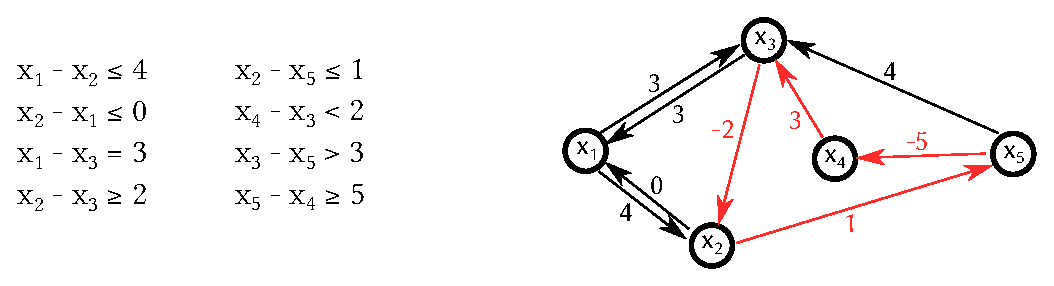
\includegraphics[width=\textwidth]{graph_unsat}
	\caption{Rozhodnutí o~nesplnitelnosti STP nalezením záporného cyklu}
\end{figure}

Tyto algoritmy však trpí pro náš účel zásadním nedostatkem. Jejich použití znamená, že po každém přidání nové hrany do grafu musí znovu proběhnout celé prohledávání. Tento postup není vhodný pro použití v~SMT řešičích, ve kterých je kladen velký důraz na inkrementalitu. V~následující sekci tedy podrobně rozebereme několik postupů pro řešení problémů SMT s~ohledem na DL a~motivujeme výběr námi použitého algoritmu. 

\section{Volba algoritmu}\label{alg}

Jak jsme ukázali v~předchozí sekci, ne všechny algoritmy na rozhodnutí STP jsou dobrou volbou pro použití v~kontextu SMT řešičů. Řešič teorie pro DPLL($T$) by měl efektivně podporovat dvě zásadní operace --- inkrementální přidávání literálů a~backtracking.

Na rozdíl od základního hladového přístupu, jak byl popsán v~\ref{smt}, v~DPLL($T$) dostává \Solver informaci o~rozhodnutých ohodnoceních průběžně. Aby byly dříve odhaleny slepé větve v~rozhodovacím stromu, \Solver je průběžně dotazován na splnitelnost dosud provedených rozhodnutí. Pro zrychlení tohoto procesu je tedy vhodné, aby byl schopen pro výpočet využít výsledků z~předchozích dokončených výpočtů. Algoritmy, které nedokáží takto zakomponovat mezivýpočet podproblému, budou ze své podstaty méně výkonné na postupné sekvenci splnitelných ohodnocení.

Po nalezení nesplnitelného ohodnocení pak neopakuje engine celý výpočet, ale vrací se pouze do nejbližšího stavu, ve kterém bylo ohodnocení ještě splnitelné. Od řešiče teorie očekáváme, že je schopen efektivně zapomínat přidané literály, vracet se do předchozích stavů a~pokračovat z~nich ve výpočtu. %% FIXME: Better wording?
S~ohledem na tyto požadavky vzniklo několik algoritmů pro řešení SMT s~ohledem na DL. V~této práci se budeme zabývat převážně postupem založeným na vyčerpávající propagaci teorie, který postulovali v~roce 2005 Nieuwenhuis a~Oliveras \cite{Nieuwenhuis05}. Ten podrobně popisujeme v~sekci \ref{dpllt}. Existují ale i~další přístupy, kterými lze v~rámci DPLL($T$) problém řešit.

Jako možnou alternativu uveďme algoritmus, který prezentovali Wang a~kol. \cite{Wang05} a~jejichž řešič se koncepčně od našeho přístupu značně liší. Vychází z~Bellman-Fordova algoritmu, využitelného mimo jiné k~detekci záporných cyklů. Pomocí několika klíčových pozorování pak odstraňuje jeho nedostatky pro použití v~SMT řešičích. Zásadní změna spočívá v~inkrementalitě řešení. Běžný Bellman-Fordův algoritmus by musel pokaždé relaxovat všechny hrany grafu nezávisle na předchozích výpočtech. Jak ale ukázali autoři \cite{Wang05}, pokud nepotřebujeme hledat nutně nejkratší cesty, nemusí vrcholy grafu nutně začínat s~nekonečným potenciálem. Jejich řešič si tedy může ukládat délky nalezené v~jednom průběhu relaxačního algoritmu a~použít je jako výchozí hodnoty pro následující průběh. Tím se v~praxi podstatně sníží počet relaxací nutných ke stabilizování všech vrcholů. Tento proces také umožňuje efektivní backtracking a~hledání splňujícího modelu.

Pro tuto práci jsme nakonec zvolili postup, který uvádějí Nieuwenhuis a Olivieras \cite{Nieuwenhuis05}, z několika důvodů. Jedním byla myšlenka vyčerpávající propagace, jejíž použitelnost v rámci OpenSMT jsme chtěli vyzkoušet. Z implementační strany nás zaujala nás také aktivnější role řešiče teorie v tomto algoritmu; zatímco řešič popsaný v předchozím odstavci je v zásadě pasivní, v námi zvoleném řešiči probíhá oboustrannější komunikace se zbytkem frameworku. Jelikož jsou navíc oba přístupy výkonostně srovnatelné \cite{Wang05}, naše rozhodnutí by nemělo negativně ovlivnit efektivitu řešení. Využití výše uvedeného řešiče a jeho srovnání se stávající implementací, popřípadě vytvoření zcela nového způsobu řešení DL v rámci DPLL($T$), vidíme jako možná budoucí rozšíření této práce.

\chapter{Popis řešení}

V~této kapitole rozebereme obecné vlastnosti našeho řešení. Nejprve detailněji popíšeme použitý algoritmus a~opodstatníme některá koncepční rozhodnutí, která jsme učinili jako důsledek použitého frameworku. Poté nastíníme obecný způsob fungování programu a~zamyslíme se nad rozdíly mezi různými variantami řešeného problému.

\section{DPLL($T$) s~vyčerpávající propagací teorie}\label{dpllt}

Připomeňme si metodu \icode{SetTrue} uvedenou v~sekci \ref{smt}. Ta slouží k~přidání nového omezení do kontextu řešiče teorie. Řešič může volitelně jako návratovou hodnotu uvést nějakou množinu literálů, které detekoval jako důsledky vzniklé přidáním právě tohoto omezení. Může přitom hlásit např. jen \uv{zjevné} důsledky, popřípadě nemusí vracet vůbec žádné. Pokud jsme je ale schopni nacházet v~rozumém čase, nahlášené důsledky jsou užitečnou informací pro hlavní engine, poněvadž pro něj mohou výrazně zmenšit velikost rozhodovacího stromu.

Varianta DPLL($T$) s~vyčerpávající propagací teorie přidává pro \icode{SetTrue} silnou podmínku; řešič musí vrátit \emph{všechny} literály ze vstupní formule, které jsou důsledky stávajícího ohodnocení. Tento předpoklad značně zjednoduší DPLL($X$) engine a~umožní mu pracovat efektivněji. Stane se z~něj \emph{de~facto} běžný SAT řešič, který se liší pouze minimalistickým rozhranním se \Solver. To má mimo jiné za důsledek, že jsme nyní schopni převézt libovolný SAT řešič na bázi DPLL do DPLL($X$) enginu.

Nevýhoda tohoto přístupu je jasná. Povinnost hledat všechny důsledky teorie může řádově zpomalit operaci \icode{SetTrue} pro řešič teorie. Nicméně se ukázalo~\cite{Nieuwenhuis05}, že alespoň v~případě diferenční logiky může tento přístup vést k~rychlé implementaci schopné předčit ostatní alternativy.

\subsection{Návrh řešiče pro diferenční logiku}

\Solver diferenční logiky využívá principy, se kterými jsme se podrobněji seznámili v~předchozích sekcích. Můžeme například předpokládat, že všechna omezení jsou tvaru $x-y \leq c$ (převod z~dalších forem jsme popsali v~sekci \ref{stp}). Využijeme též převodu omezení do tvaru omezujícího grafu, jak bylo uvedeno v~sekci \ref{graf}.

\subsubsection*{Inicializace}
Během inicializace načte řešič vstupní formuli, uloží si všechna rozdílová omezení, která se v~ní vyskytují, a~předá ji DPLL($X$) jako čistě booleovskou formuli. Během tohoto procesu by měl detekovat vztahy mezi literály a~jejich negacemi a~explicitně je poznamenat. Pokud se například na vstupu vyskytnou nerovnice $x-y \leq 1$ a~$y-x \leq -2$, v~oboru celých čísel je jedna negací druhé. Řešič by tak měl abstrahovat tyto výskyty jako $p$ a~$\neg p$ pro booleovskou proměnnou $p$. Ukládá si přitom překladovou tabulku pamatující si pro každou nerovnici abstrahovaný literál, kterému odpovídá. Zároveň s~tím si udržuje pro každou proměnnou seznam všech nerovnic, ve kterých se tato proměnná vyskytuje (účel těchto seznamů je objasněn níže).

\subsubsection*{Ohodnocení literálu}
Jakmile je následně nastavena pravdivostní hodnota některého literálu, převede jej řešič do formy $x-y \leq c$ a~přidá odpovídající hranu do omezujícího grafu. Následně musí objevit všechny důsledky tohoto ohodnocení. Pro jejich nalezení je potřeba zkontrolovat všechny cesty $$x_i \xrightarrow{c_i*} x \xrightarrow{c} y \xrightarrow{c'_j*} y_j$$ a~zjistit, zda nějaké omezení neplyne z~$x_i - y_j \leq (c_i + c + c'_j)$. To budou právě nerovnice tvaru $x_i - y_j \leq c'$, kde $c' \geq c_i + c + c'_j$. 

Abychom prošli všechny tyto cesty procházející nově přidanou hranou, musíme nejdřív nalézt seznam všech vrcholů $x_i$, ze kterých je dosažitelné $x$, a~seznam všech vrcholů $y_j$, které jsou dosažitelné z~$y$. Omezující graf je tedy reprezentován jako oboustranný seznam sousedů. Potom už můžeme spustit obyčejný algoritmus na hledání nejkratší cesty, kterým získáme všechna vhodná $x_i$ společně s~jejich $c_i$, resp. $y_j$ s~jejich $c'_j$. Autoři \cite{Nieuwenhuis05} pro toto prohledávání doporučují následující postup.

Použijeme běžné prohledávání do hloubky. V~něm si označíme každý vrchol, který jsme navštívili poprvé, společně s~jeho vzdáleností. Navštívíme-li pak již objevený vrchol znovu, pokračujeme v~prohledávání pouze tehdy, když je jeho současná vzdálenost menší než naše uložená vzdálenost. Zároveň si všechny objevené $x_i$ a~$y_j$ ukládáme do dvou odlišných seznamů. Po skončení prohledávání spočteme pro oba seznamy počet všech nerovnic, ve kterých se proměnné v~seznamu vyskytují (tyto nerovnice si pro každou proměnnou pamatujeme z~inicializace).

Vyskytují-li se potom například $x_i$ celkově v~menším počtu proměnných, projdeme pro každé $x_i$ seznam všech nerovnic, ve kterých se vyskytuje, a~zkontrolujeme, zda se nejedná o~důsledek nalezené cesty z~$x_i$ do nějakého $y_j$.

\subsubsection*{Hledání příčin}

Jak víme z~\ref{smt}, řešiče teorie musí implementovat operaci \icode{Explain}, která pro nalezený důsledek vrátí množinu jeho příčin. Tato operace je důležitá pro budování implikačního grafu v~DPLL($X$) a~určení vhodné úrovně backtrackingu při nalezení sporu. Řešič DL popsaný v~\cite{Nieuwenhuis05} tuto operaci provádějí následovně.

Když je do omezujícího grafu přidána $n$-tá hrana, zapamatujeme si k~této hraně její odpovídající $n$. U~nalezených důsledků si pamatujeme $n$ hrany, jejímž přidáním důsledek vznikl. Když pak hledáme vysvětlení hrany $h$ tvaru $x-y \leq c$, spustíme prohledávání z~$x$ do $y$ stejným způsobem jako po přidání hrany. Prohledávání ale pouštíme jen do délky nejvýše $c$ a~jen přes hrany s~číslem vložení nejvýše $n$. Tato omezení zvyšují efektivitu (zmenšujeme prostor k~prohledání) a~zaručují, že nepoužíváme hrany přidané až po důsledku (což by působilo problémy v~implikačním grafu DPLL($X$)). Nalezená cesta tak má délku kratší nebo rovnou $c$ a~sestává se jen z~dříve přidaných hran, z~čehož jasně vidíme, že $h$ je důsledek hran na této cestě.

\section{Úpravy referenčního algoritmu}\label{upravy}

Naše implementace je převážně založená na algoritmu tak, jak ho postulovali Nieuwenhuis a~Oliveras \cite{Nieuwenhuis05}. Přesto se liší v~některých implementačních detailech, daných zejména odlišnostmi OpenSMT od referenčního DPLL($T$) frameworku. %% TODO finish

Prvním důležitým rozdílem je způsob abstrakce literálů teorie. V~OpenSMT neexistuje způsob, kterým bychom mohli informovat hlavní engine o~vztazích mezi různými nerovnicemi. Obsahuje-li například vstupní formule nerovnice $(x-y\leq 3)$ a~$(y-x<-3)$, algoritmus popsaný v~\cite{Nieuwenhuis05} je pro DPLL($X$) abstrahuje do booleovských symbolů $p$ a~$\neg p$. Této abstrakce nejsme pomocí rozhranní v~OpenSMT schopni. Náš řešič si tedy musí tyto vztahy udržovat interně. 

S~tímto omezením úzce souvisí druhý zásadní rozdíl. Můžeme si všimnout, že schéma uvedené v~sekci \ref{smt} umožňuje frameworku ohodnotit literál pouze jako \emph{true}. Uvědomme si, že to obecně není nijak omezující. Ohodnocení termu $p$ jako \emph{false} totiž můžeme snadno zařídit voláním \icode{SetTrue($\neg p$)}. Protože však OpenSMT nezná tato mapování mezi termy a~jejich negacemi, není pro nás tento přístup validní. Namísto toho využíváme přímočařejší implementace, kde termům můžeme přiřadit ohodnocení \emph{true} i~\emph{false}. Tato odlišnost vyžaduje několik modifikací našeho řešiče. 

Předně musíme být schopni detekovat, zda jedna nerovnice neodpovídá negaci druhé, jak už jsme uvedli výše. Jakmile jsme toho schopni, můžeme záporné ohodnocení hrany implementovat jako přidání negace této hrany do omezujícího grafu. Jak ale postupovat, pokud jsme u~některé hrany tuto negaci nenašli? Naivní přístup by byl vytvořit negaci takové hrany ve chvíli, kdy se objeví její záporné ohodnocení. Takové řešení však není možné: uvažujme neohodnocenou hranu $h$, která ve vstupní formuli nemá svou negaci. Mějme dále v~omezujícím grafu nějakou množinu hran $M$ takovou, že $M \cup \{h\}$ tvoří záporný cyklus. Pokud $M$ existuje, očividně je $\neg h$ důsledkem tohoto grafu. Jelikož se ale $\neg h$ nevyskytuje ve vstupní formuli a~$h$ nebyla nikdy záporně ohodnocená, nevyskytuje se $\neg h$ v~seznamu možných hran našeho řešiče. Algoritmus hledání důsledků ji tudíž nemůže nalézt. Kladným ohodnocením $h$ potom vytvoříme záporný cyklus v~omezujícím grafu, čímž porušíme invariant našeho algoritmu a~nekonečně zacyklíme příští hledání důsledků.

Jak vidíme, negace všech hran musí být známy předtím, než proběhne prohledávání grafu. Tento problém jsme se tedy rozhodli vyřešit už při oznamování možných literálů. Když je řešiči předán literál vyskytující se ve formuli, vytvoříme nejen hranu odpovídající tomuto literálu, ale okamžitě i~hranu odpovídající její negaci. Při předávání dalších literálů je pak jen třeba ověřit, zda neodpovídají některé již vytvořené hraně. Podrobněji tento postup popisujeme v~sekci \ref{add}.

Za zmínku stojí také to, že OpenSMT nevyžaduje nutně kontrolu konzistence po každém ohodnocení. Tuto možnost ponechává řešičům pouze volitelně a~přidává do rozhranní operaci \icode{Check}, pomocí které kontrolu explicitně vyvolává. Může tím sice způsobit, že nějakou dobu pokračuje s~hodnocením proměnných v~nekonzistentním stavu, ale na druhou stranu tím lze dosáhnout vyšší efektivity, pokud je v~dané teorii kontrola náročnou operací. Jelikož referenčním algoritmem dokážeme triviálně detekovat sporná ohodnocení (\ref{rozhod}), náš řešič o~nich informuje vždy již při jejich oznámení. Z~\icode{Check} se pak stává prázdná operace, která jen vrací současný stav řešiče.

Posledním větším rozdílem je způsob zpracování konfliktů. Jedním z~důsledků vyčerpávající propagace je fakt, že řešič nemusí kontrolovat nesplnitelnost předaného ohodnocení. Zapříčinilo-li by přidání nějaké hrany spor, negace této hrany je důsledkem omezujícího grafu. Můžeme přitom předpokládat, že DPLL($X$) negaci objeveného důsledku nikdy řešiči nepředá. OpenSMT se v~tomto ohledu liší ve způsobu, jakým analyzuje sporný stav. Jeho řešiče obecně nepodporují operaci \icode{Explain}, vracející pro nějaký důsledek množinu jeho příčin. Místo toho implementují funkci \icode{getConflict}, která hledá nesplnitelnou množinu literálů. Pro použití této funkce, nutné k~určení úrovně backtrackingu, se ale nejdřív musí řešič dostat do nekonzistentního stavu.

Tyto dva přístupy jsou naštěstí ekvivalentní. Když OpenSMT objeví spor, předá řešiči nějaké zaručeně sporné ohodnocení, čímž ho dostane do nekonzistentního stavu. Z~tohoto důvodu musíme před každým přidáním hrany kontrolovat, zda není sporná se stávajícím ohodnocením (více viz.~\ref{add}). Náš řešič si zapamatuje hranu $h$ odpovídající tomuto ohodnocení a~funkce \icode{getConflict} pak odpovídá volání \icode{Explain($\neg h$)}. 

\section{Popis běhu programu}

\begin{figure}
	\centering
	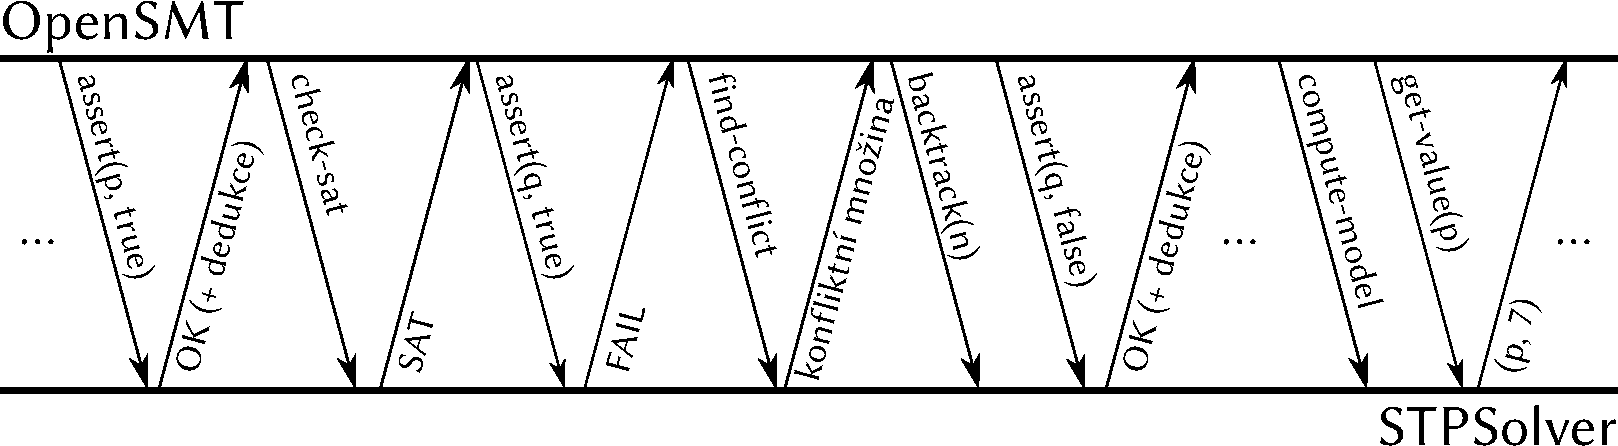
\includegraphics[width=\textwidth]{interface}
	\caption{Ukázka interakce řešiče s~OpenSMT (pseudokód)}
\end{figure}

V~první fázi algoritmu jsou řešiči předány všechny literály teorie, které se vyskytují ve vstupní formuli. Řešič z~nich nejprve extrahuje relevantní hodnoty. Následně zkontroluje, zda se nejedná o~negaci některého z~již zapamatovaných literálů. Pokud ano, pouze tuto negaci explicitně označí. V~opačném případě vytvoří hranu odpovídající tomuto literálu a~zároveň a~priori hranu tvořící negaci tohoto literálu, jak je popsáno v~sekci \ref{upravy}. Obě nové hrany se stanou součástí úložiště a~jsou zařazeny do překladových tabulek. Zbytek výpočtu pak již může předpokládat, že pracujeme pouze se známými literály, pro něž máme vytvořené hrany.

Poté, co jsou všechna omezení načtena, nastává hlavní část programu. Během té postupně řešič dostává rozhodnutá ohodnocení literálů. Když nějaké obdrží, přidá do omezujícího grafu hranu odpovídající tomuto ohodnocení. Následně proběhne prohledávání objevující všechny důsledky tohoto ohodnocení. Tyto důsledky jsou přeloženy zpět do vhodné formy a~oznámeny frameworku.

Po nějaké sekvenci těchto ohodnocení buď nalezneme splňující ohodnocení celé formule, nebo se dostaneme do sporu. Spor můžeme rozpoznat tak, že se chystáme přidat do grafu hranu, jejíž negace byla buď dříve do grafu přidána, nebo byla nalezena jako důsledek dřívějšího ohodnocení. V~takovém případě řešič oznámí selhání tohoto ohodnocení a~přejde do chybového stavu. Jakmile je řešič v~chybovém stavu, automaticky zamítá všechna nová ohodnocení. V~této situaci následuje nalezení nesplnitelné množiny. Pokud byla objevená negace hrany explicitně přidána do grafu, je tato množina triviální. Jinak ji získáme modifikovanou verzí prohledání grafu (viz.~\ref{alg}). Jakmile je nesplnitelná množina nalezena a~předána frameworku, rozhodne se podle ní úroveň backtrackingu. Ten je v~OpenSMT řešen obecně pomocí systému záchytných bodů. Řešič může být v~libovolnou chvíli požádán, aby uložil svůj aktuální stav na zásobník. V~případě nutnosti je mu pak sděleno, aby odebral několik bodů z~vrchu tohoto zásobníku a~tím se vrátil do dřívějšího stavu. 

Jakmile se řešič vrátí do konzistentního stavu, tento proces se opakuje, dokud není nalezeno nějaké splnitelné ohodnocení, nebo dokud framework nevyčerpá všechny možnosti ohodnocení. Splnitelnost formule je určena tím, který z~těchto dvou případů nastane. V~případě, že je formule splnitelná, může být řešič na závěr výpočtu ještě požádán, aby vytvořil její model, tedy nalezl konzistentní hodnoty pro všechny proměnné obsažené v~literálech teorie.

\section{Srovnání reálné a~celočíselné verze} \label{int_v_real}

Algoritmus uvedený v~sekci \ref{alg} je s~drobnými úpravami použitelný jak pro RDL, tak pro IDL. Přestože v~této práci implementujeme pouze celočíselnou verzi problému, přišlo nám názorné zamyslet se nad rozdíly mezi oběma variantami.

%Uveďme nejprve pro zajímavost, že pokud na vstupu podporujeme i~rovnice a~jejich negace, ověření konzistence je možné v~reálných číslech provést polynomiálně, zatímco pro celožíselný obor je ověření NP-těžké --- jsme schopni na něj převést např. problém $k$-barevnosti grafu \cite{slides}.

Prvním zjevným rozdílem pro potřeby naší implementace je reprezentace čísel. Reálná čísla je potřeba reprezentovat jinak, než čísla celá. OpenSMT definuje vlastní datový typ pro reálná čísla nazvaný \icode{FastRational}. V~různých částech kódu jej můžeme najít také pod aliasy \icode{Real} nebo \icode{Number}. Tento typ má několik výhod oproti běžným primitivním typům s~pohyblivou desetinnou čárkou. Především se jedná o~typ s~teoreticky neomezenou velikostí. Jelikož využívá struktur větších než jedno procesorové slovo, není limitován kapacitami procesoru. Důsledkem toho je to také typ s~libovolnou přesností. Netrpí tak zaokrouhlovacími chybami a~ztrátou platných číslic u~velkých hodnot jako např. \icode{float} a~\icode{double}. Tyto vlastnosti jsou důležité, jelikož sémantika SMT-LIB\footnote{sada standardů a~knihoven zabývající se SMT řešiči, vůči níž je OpenSMT implementováno} vyžaduje, aby všechny číselné výpočty probíhaly s~neomezenou přesností.

Samozřejmě bychom mohli \icode{FastRational} použít i~v~celočíselném řešení. Usnadnilo by nám to návrh datových struktur a~umožnilo větší znovupoužitelnost kódu. Testováním se však ukázalo, že aritmetické operace na \icode{FastRational} jsou citelně pomalejší než u~primitivních typů. Náš projekt tak používá primitivní celočíselný typ, konkrétně typ \icode{ptrdiff\_t}\footnote{\icode{ptrdiff\_t} byl vybrán jako znaménkový typ s~největším rozsahem, který můžeme na cílové architektuře očekávat}. Ten bohužel podporuje pouze hodnoty omezeného rozsahu a~je tak v~rozporu se standardem. Protože ale v~OpenSMT zatím neexistuje ekvivalent \icode{FastRational} pro celá čísla, uznali jsme jej jako nejlepší volbu. Toto rozhodnutí bylo podpořeno skutečností, že omezení rozsahu se experimentálně ukázalo jako zanedbatelné pro běžné použití --- z~661 testů knihovny SMT-LIB náš řešič vrátil ve všech případech správný výsledek (podrobněji viz.~kapitola \ref{experiment}).

Zásadní algoritmický rozdíl je také v~tvorbě negací. Máme-li například na vstupu nerovnici $(x-y<k)$, v~IDL ji triviálně převedeme do tvaru $(x-y\leq k-1)$. V~RDL se ovšem ostrých nerovností tak snadno nezbavíme. Nieuwenhuis a~Olivieras \cite{Nieuwenhuis05} navrhují pro tento případ postup, který využili např. Dutertre a~de Moura ve svém řešiči pro lineární aritmetiku \cite{Dutertre06}. Ten je založen na následujícím tvrzení.
\begin{tvrz}[Dutertre a~de Moura \cite{Dutertre06}, Lemma 1] 
	Nechť množina literálů lineární aritmetiky $\Gamma$ obsahuje ostré nerovnosti $S = \{p_1 > 0,\dots,p_n > 0\}$. $\Gamma$ je splnitelná právě tehdy, když existuje racionální $\delta > 0$ takové, že $\Gamma_\delta = (\Gamma \cup S_\delta) \setminus S$ je splnitelná, kde $S_\delta = \{p_1 \geq\delta,\dots,p_n \geq\delta\}$.
\end{tvrz}

Toto tvrzení umožňuje nahradit všechny ostré nerovnice neostrými, známe-li dostatečně malé $\delta$. Hodnotu $\delta$ přitom Dutertre a~de Moura nepočítají přímo, ale používají ho pouze symbolicky jako \emph{infinitesimální parametr}. Omezení a~proměnné pak nejsou ohodnoceny běžnými racionálními čísly, ale dvojicemi čísel $(c, k)$, reprezentujícími výraz $c + k\delta$, na kterých zavedeme odpovídající aritmetické a~porovnávací operace. Vhodnou substituci za $\delta$ je po této substituci třeba hledat až na samotném konci výpočtu, pokud chceme najít model spňujícího ohodnocení. V~kontextu OpenSMT už je tento přístup použit rovněž v~řešiči teorie lineární aritmetiky.

Na závěr ještě připomeňme omezení týkající se datových struktur použitých v~OpenSMT. Jelikož \icode{FastRational} obsahuje ukazatele, nelze jej --- ani typy, které ho obsahují --- použít například jako prvek třídy \icode{vec}. Na tato omezení je třeba dbát při přechodu z~celočíselné verze na reálnou.

\chapter{Vývojová dokumentace}
V~této kapitole se budeme detailněji věnovat implementaci našeho řešení. Rozebereme její strukturu, jednotlivé části programu a~rozhodnutí, která bylo potřeba učinit. Po přečtení kapitoly by měl být čtenář schopen orientovat se v~našem řešení a~rozumět účelu jeho jednotlivých částí. Podrobně též popíšeme zapojení řešiče do infrastruktury OpenSMT.

Vzhledem k~povaze řešení jakožto interní součásti většího frameworku neobsahuje tato práce uživatelskou dokumentaci. Návod na spuštění OpenSMT a~názornou ukázku jeho použití na problému využívajícím náš řešič nalezneme v~přílohách \ref{content}~a~\ref{priklad}.
\section{Datové struktury}\label{data}

\subsection*{Struktury OpenSMT}
Základní datovou strukturou v~OpenSMT je \icode{Pterm}, reprezentující jeden term vyskytující se ve vstupní formuli. Odkazy na tyto termy jsou pak předávány pomocí referenční struktury \icode{PTRef}. Ta obsahuje pouze numerický identifikátor použitý k~jejímu rozlišení. Mapování jednotlivých referencí na odpovídající termy přitom zařizuje třída \icode{Logic}, respektive její potomci. \icode{Logic} si ukládá převodní tabulku párující \icode{PTRef} a~jejich odpovídající \icode{Pterm} a~poskytuje také mechanismy pro vytváření nových termů. Její potomci pak rozšiřují tyto mechanismy o~možnosti odpovídající dané teorii, např. s~\icode{LALogic} jsme schopni vytvářet termy odpovídající nerovnicím z~lineární aritmetiky. Jelikož rozdílová omezení jsou specifickým tvarem lineárních nerovnic, využívá náš řešič právě schopností \icode{LALogic}, konkrétně \icode{LIALogic} pro implementovanou celočíselnou verzi.

Ohodnocení proměnných je uloženo ve struktuře \icode{PtAsgn}, která obsahuje \icode{PTRef} odpovídající ohodnocené proměnné a~\icode{lbool} označující její ohodnocení (\icode{lbool} je běžný optional boolean).

Samotné termy mají stromovou strukturu. Pokud se nejedná o~atomickou proměnnou, reprezentuje term nějaký $n$-ární funkční či relační symbol společně s~jeho argumenty. K~rozlišení typu symbolu nám opět poslouží API třídy \icode{Logic}, pro přístup k~argumentům je pak použit operátor \icode{[]}. Reprezentuje-li například \icode{Pterm~p} term $(x \lor y)$, budeme mít přístup k~proměnným \icode{p[0]} a~\icode{p[1]}, což jsou \icode{PTRef} reprezentující $x$, respektive $y$. 

\begin{code}[label=Příklad práce s~termem p $\approx (4 \leq x)$]
PTRef p;    
assert( logic.isNumLeq(p) );
Pterm &term = logic.getPterm(p);

PTRef c = term[0];
assert( logic.isNumConst(c) );
opensmt::Number n = logic.getNumConst(c);
assert( n == 4 );

PTRef x = term[1];
assert( logic.isNumVar(x) );
\end{code}

Je vhodné zmínit, že za dobu vývoje OpenSMT v~něm vzniklo několik implementací základních datových struktur. Hojně užívaným příkladem je třída \icode{vec}, reprezentující běžný vektor. Vyjma malých rozdílů API a~údajné vyšší efektivity na primitivních typech se tyto třídy výrazně neliší od implementací ze standardní knihovny. Konkrétně třída \icode{vec} je navíc omezena skutečností, že jejími prvky nemohou být typy obsahující odkazy (výjimkou z~tohoto pravidla je zvlášť implementovaný \icode{vec$\langle$vec$\langle$T$\rangle\rangle$}). Za účelem konzistence se zbytkem frameworku jsme se přesto rozhodli využívat tyto lokální implementace struktur všude, kde je to možné. 

\subsection*{Struktury řešiče}
Nejdůležitější datovou strukturou našeho řešiče je \icode{Edge}. V~té jsou uloženy informace o~jedné hraně omezujícího grafu. Konkrétně tedy obsahuje reference na její vstupní a~výstupní vrchol, ohodnocení, odkaz na svou negaci a~informaci o~tom, kdy byla přidána do omezujícího grafu. Po vzoru frameworku přitom zbytek řešiče nepracuje přímo s~těmito strukturami, ale s~jejich referencemi \icode{EdgeRef}, které opět obsahují pouze jednoznačný numerický identifikátor. Samotné hrany se pak nacházejí jen v~centrálním úložišti, které tvoří třída \icode{STPStore}. Ta zařizuje zejména tvorbu nových hran a~převod z~\icode{EdgeRef} na \icode{Edge\&}. Použit je i~protějšek k~\icode{EdgeRef} pro vrcholy, struktura \icode{VertexRef}. Jelikož se však s~vrcholy nepojí žádná informace, nejedná se o~odkaz na další strukturu, ale pouze o~symbolické reference, sloužící pro vzájemné rozlišení jednotlivých vrcholů.

%\captionof{verbatim}{test}
\begin{code}[label=Deklarace struktury Edge]
struct Edge {
    VertexRef from, to;    
    EdgeRef neg;           
    ptrdiff_t cost;
    uint32_t setTime;
}
\end{code}

Jelikož náš řešič dostává od frameworku informace o~proměnných zásadně jako \icode{PTRef}, potřebujeme způsob, jak přecházet mezi reprezentací frameworku a~interní reprezentací našeho řešiče. K~tomuto účelu slouží třída \icode{STPMapper}. V~této třídě se vyskytuje hned několik druhů převodních tabulek. Pamatuje si převod z~\icode{PTRef} na \icode{VertexRef}, přiřazující proměnné k~vrcholům grafu, a~převod z~\icode{PTRef} na \icode{EdgeRef}, přiřazující nerovnice k~hranám. Tyto převody jsou zásadní pro interpretaci příkazů frameworku. Pro hrany si pamatuje i~opačný převod, mapující \icode{EdgeRef} zpět na odpovídající \icode{PTRef}. Ten je důležitý pro oznámení nalezených dedukcí (viz.~\ref{dusl}). Pro účely oznámení nesplnitelné množiny literálů si pro hrany právě v~grafu pamatujeme i~mapu z~\icode{EdgeRef} na \icode{PtAsgn}, které způsobily jejich přidání do grafu. Uvědomme si, že tento převod není zaměnitelný s~předchozím převodem na \icode{PTRef}, jelikož hrana se může vyskytnout v~grafu z~důvodu záporného ohodnocení její negace. \icode{STPMapper} si navíc pamatuje pro každý vrchol seznam všech hran, ve kterých se daný vrchol vyskytuje, jak je popsáno v~\ref{alg}.

Samotný omezující graf ukládáme do struktury \icode{STPEdgeGraph}. Ta obsahuje seznam přidaných hran a~oboustranný seznam sousedů pro všechny vrcholy grafu. S~grafem přímo manipuluje třída \icode{STPGraphManager}, která působí jako hlavní výpočetní třída řešiče. Provádí přidávání hran do grafu a~jejich případné odebírání z~grafu, ale i~hledání důsledků přidané hrany a~hledání vysvětlení nalezeného důsledku.

Třídu \icode{STPModel} využijeme, pokud chceme pro splnitelnou množinu nerovnic najít nějaké ohodnocení proměnných. \icode{STPModel} dostane kopii grafu, ze které vytvoří mapu ohodnocení obsažených vrcholů.

Všechny struktury řešiče spojuje dohromady hlavní třída \icode{STPSolver}. Jakožto potomek \icode{TSolver} implementuje tato třída rozhraní mezi řešičem a~zbytkem frameworku. Vztahy mezi jednotlivými strukturami řešiče shrnuje obrázek \ref{fig:deps}.
\begin{code}[labelposition=bottomline,label=Základní API třídy STPSolver]
class STPSolver : public TSolver {
public:
	void declareAtom(PTRef tr);
	bool assertLit(PtAsgn asgn);
	TRes check(bool b);
	void getConflict(vec<PtAsgn> &vec);
	void pushBacktrackPoint();
	void popBacktrackPoints(unsigned int i);
	void computeModel();
	ValPair getValue(PTRef pt);
}
\end{code}

\begin{figure}
	\centering
	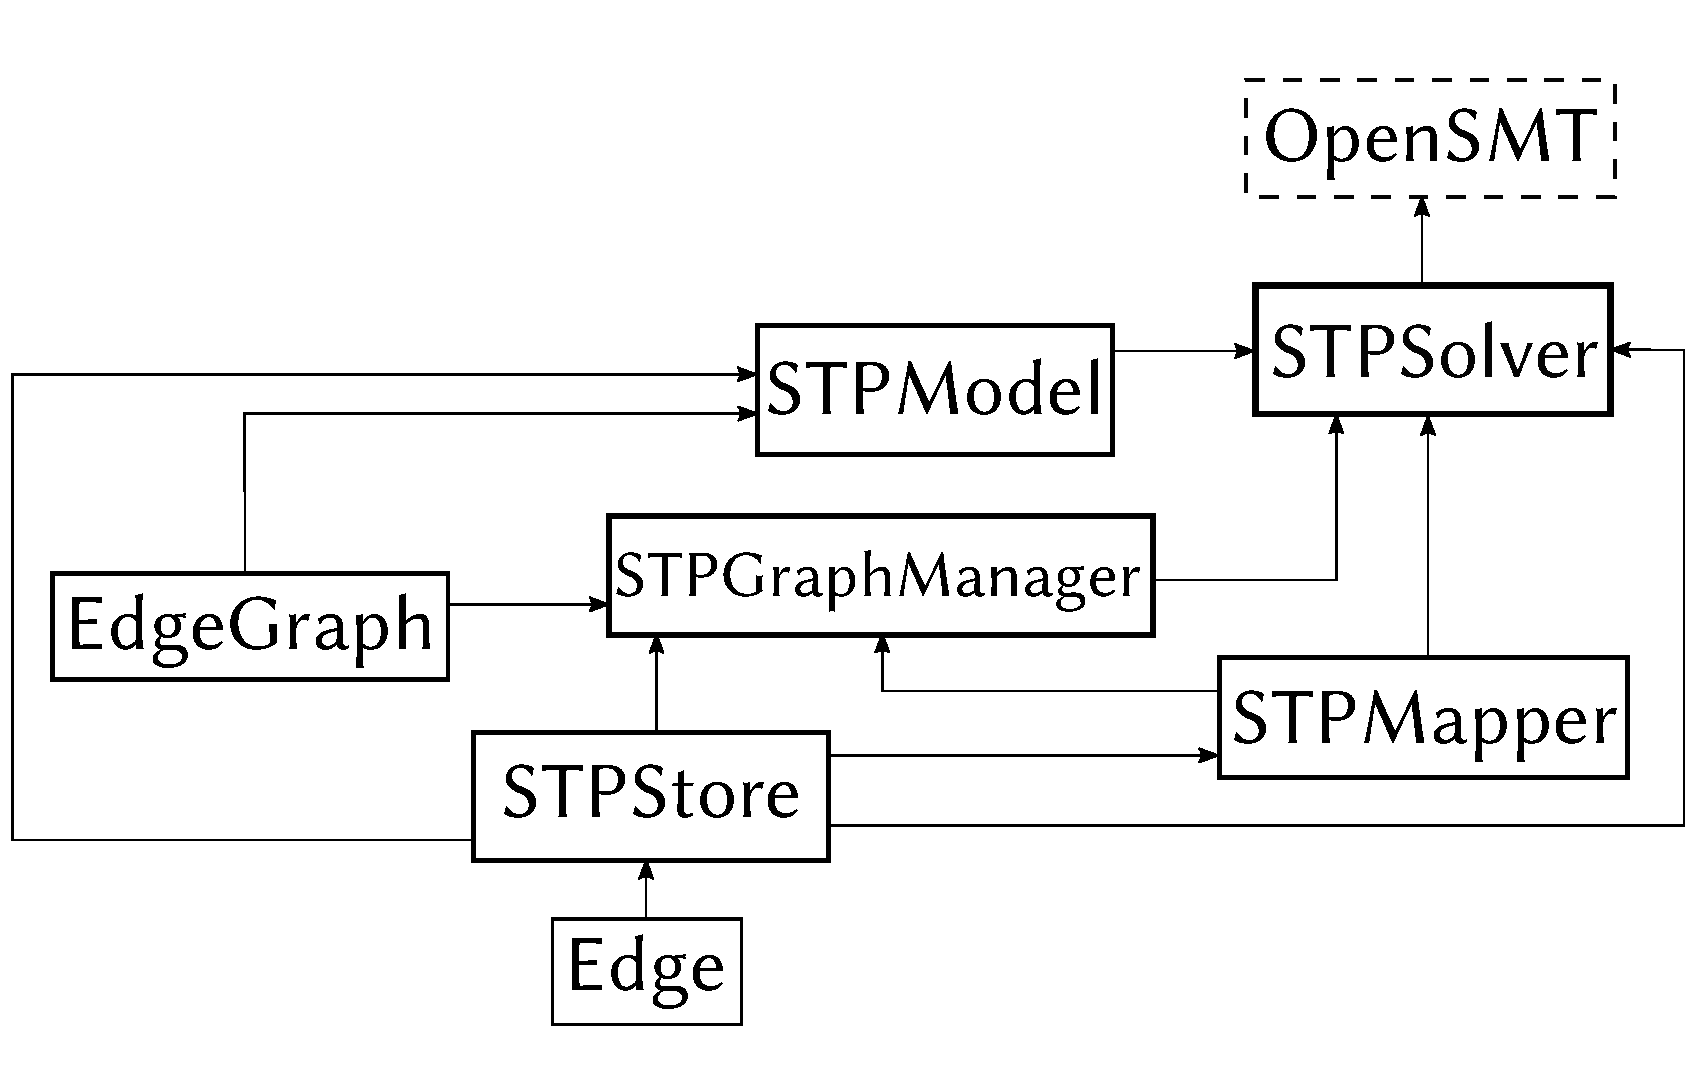
\includegraphics[width=0.8\textwidth]{class_deps}
	\caption{Závislosti mezi strukturami řešiče}
	\label{fig:deps}
\end{figure}

\section{Přidávání literálů}\label{add}

Na samotném začátku výpočtu se OpenSMT postupně pro každý term zeptá řešiče, zda se jedná o~literál jeho teorie. Jelikož tento proces slouží primárně k~jejich odlišení od běžných booleovských termů, nezkoumáme do hloubky struktury termu, ale provádíme jen povrchovou kontrolu. Pokud předpokládáme, že framework použije náš řešič jen pro odpovídající teorii, je taková kontrola dostačující.
\begin{code}
bool STPSolver::isValid(PTRef tr) { return logic.isNumLeq(tr); }
\end{code}

Jakmile jsou termy takto rozlišeny, řešič je informován o~všech literálech, jejichž ohodnocení mu může být oznámeno. K~tomu je využita funkce \icode{declareAtom(PTRef)}. V~té už musíme projít strukturu literálu, abychom z~něj extrahovali relevantní informace. Důležité pro nás přitom je, že díky způsobu, kterým OpenSMT vytváří své termy, nemusíme provádět konverze z~různých tvarů omezení (popsaných v~sekci \ref{stp}). Neostrých nerovností a~obrácených znamének jsme tak v~literálech zbaveni dříve, než se o~nich řešič vůbec dozví --- všechny literály naší teorie jsou reprezentovány standardní formou $c \leq x - y$, popř. $c \leq \pm x$ pro omezení s~jednou proměnnou.\footnote{Tato kanonická transformace mimo jiné ospravedlňuje výše zmíněnou implementaci \icode{isValid}.} Uveďme pro úplnost, že rozdíl je v~této reprezentaci nahrazen součtem záporu. Přesnější popis struktury literálu tak je spíše $c \leq x + (-1 \cdot y)$, což můžeme vidět i~na obrázku \ref{fig:term}.

Z~této formy nám už nedělá problém určit hodnotu $c$ a~reference na $x$ a~$y$ postupem naznačeným v~předchozí sekci. Musíme přitom dbát pouze na to, že nerovnice je v~opačné formě než té námi používané. Hrany omezujícího grafu tudíž povedou z~$y$ do $x$ s~ohodnocením $-c$. Tuto odlišnost zdůrazňujeme, protože je v~implementaci práce použití identifikátorů \icode{x} a~\icode{y} standardizováno ve smyslu cílového, resp. zdrojového vrcholu hrany.

\begin{figure}
	\centering
	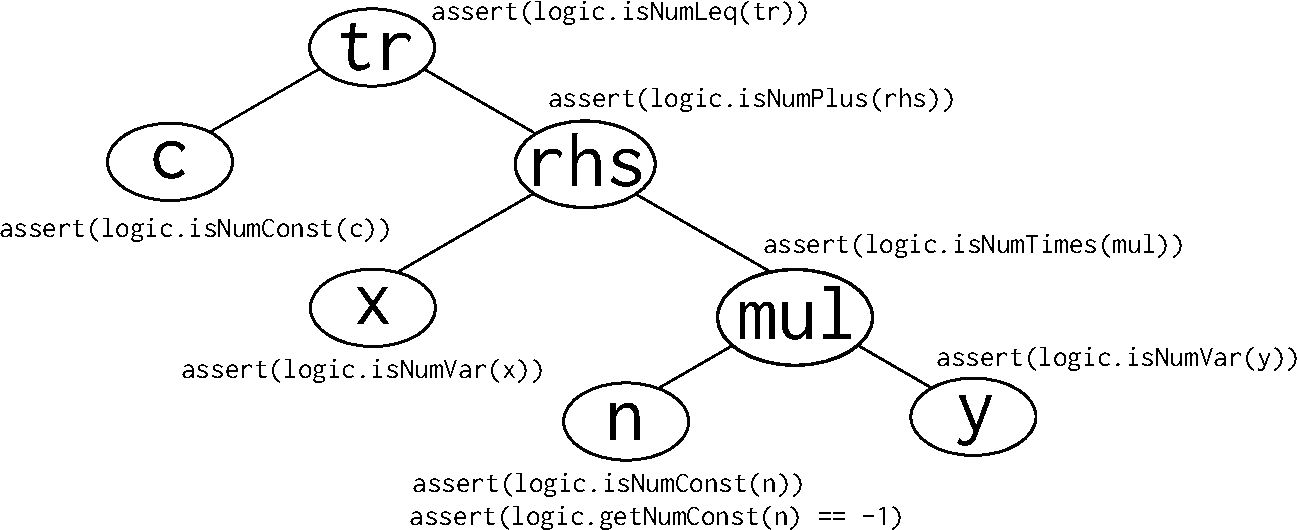
\includegraphics[width=\textwidth]{ptref_structure}
	\caption{Ukázka struktury termu (\icode{PTRef tr} $\approx c \leq x - y$)}
	\label{fig:term}
\end{figure}

Jakmile jsme získali informace o~hraně, musíme nejprve zkontrolovat, zda už hrana v~našem řešiči neexistuje. To se může stát, pokud je hrana negací jiné již přidané hrany (viz. níže). %% TODO garbage reference
Hledání hrany probíhá postupným projitím seznamu všech hran, ve kterých se vyskytuje $y$ (seznamy si pro každý vrchol ukládá \icode{STPMapper}). Probíhá tedy lineárně v~počtu hran obsahujících $y$. Jelikož ale přidávání literálů celkově zabírá jen minimální část celého výpočtu, usoudili jsme, že lineární složitost této operace je pro nás přijatelným kompromisem.

Objevíme-li hranu odpovídající přidanému literálu, stačí nám přidat do třídy \icode{STPMapper} tuto asociaci. Všechny ostatní informace o~hraně už známe. V~opačném případě musí ze všeho nejdříve \icode{STPStore} tuto hranu vytvořit (případně s~vrcholy, které jsme ještě nepotkali). Jakmile je hrana vytvořená, vytvoříme předběžně i~její negaci (z~důvodů popsaných v~sekci \ref{upravy}). Obě nově vytvořené hrany pak přidáme do seznamů hran pro jejich vrcholy. U~původní hrany si navíc uložíme její asociaci s~oznámeným literálem (pro negaci zatím tato asociace neexistuje). 

Poté, co tento proces proběhne pro všechny literály ve vstupní formuli, jsme schopni každý literál převézt na odpovídající hranu a~naopak a~dokážeme reprezentovat libovolné ohodnocení přidáním odpovídající hrany do omezujícího grafu.

\section{Oznámení ohodnocení a~hledání důsledků}\label{dusl}

Nejdůležitější část výpočtu se odehrává ve funkci \icode{STPSolver::assertLit}, pomocí které se řešič dozvídá o~nových ohodnoceních literálů. Funkce nejprve zkontroluje, zda se řešič nenachází ve sporném stavu. Pokud ano, přidávání další hrany nemá smysl a~funkce okamžitě skončí neúspěchem. V~opačném případě převedeme ohodnocení na odpovídající hranu. Následně si uložíme asociaci hrany s~danou proměnnou \icode{PtAsgn}, přidáme ji do omezujícího grafu a~začneme hledat důsledky tohoto přidání. Přidání hrany do grafu znamená její přidání do seznamu hran grafu a~do obou seznamů sousedů a~nastavení její vlastnosti \icode{setTime} na počet aktuálně přidaných hran.

Hledání důsledků zařizuje funkce \icode{STPGraphManager::findConsequences}. Ta nejprve najde seznam možných počátečních a~koncových vrcholů pro cesty procházející přidanou hranou. K~tomu využíváme prohledávání do hloubky, jak bylo popsané v~referenčním algoritmu (\ref{alg}). Prohledávání přitom probíhá sekvenčně --- nejprve hledáme počáteční vrcholy, poté hledáme vrcholy cílové. Jelikož prohledávání na společných datech provádí pouze čtecí operace, bylo by možné tento proces paralelizovat a~hledat obě množiny současně. Během vývoje jsme zkoušeli uplatnit tento přístup, nicméně režie vytváření a~rušení vláken  se ukázala časově náročnější než samotné prohledávání. Prozkoumali jsme také možnost nastavit hranici na velikost grafu určující, zda výpočet proběhne sekvenčně, či paralelně. V~praxi se ale ukázalo, že hranice byla buď příliš vysoká a~vícevláknový přístup nebyl nikdy použit, nebo byla příliš nízká a~použití vláken stále zhoršovalo výkonnost programu. Rozhodli jsme se tak zůstat u~běžné jednovláknové varianty. Využití perzistentního pole vláken nebo rigoróznější hledání limitu pro použití vlákna jsou možné oblasti dalšího zkoumání, dle našeho úsudku by ale nepřinesly podstatné zrychlení algoritmu.

Poté, co obě množiny nalezneme, vybereme tu, jejíž vrcholy se celkově objevují v~menším množství hran (tyto součty počítáme v~průběhu DFS). Pro každý vrchol z~vybrané množiny projdeme seznam všech hran, v~nichž se vyskytuje (tyto seznamy si ukládá \icode{STPMapper}) a~uložíme si všechny, které jsou důsledky naposledy přidané hrany. Aby byla hrana $a \xrightarrow{c'} b$ důsledkem právě přidané hrany $y \xrightarrow{c} x$, musí platit 
\begin{enumerate}
	\item Existuje cesta $a \rightarrow y \xrightarrow{c} x \rightarrow b$.
	\item $c'$ je větší než délka nejkratší takové cesty.
\end{enumerate}

Snadno nahlédneme, že tyto dvě podmínky pokrývají právě všechna omezení, která jsou důsledky přidání hrany $y \xrightarrow{c} x$ do grafu. Jakmile objevíme všechny takovéto hrany, musíme je převézt zpět do tvaru \icode{PtAsgn} a~předat je frameworku. Odpovídá-li přitom hraně \icode{h} literál \icode{tr} a~negaci \icode{h} literál \icode{nr}, objevení \icode{h} jakožto důsledku způsobí označení \icode{PtAsgn(tr,true)} a~\icode{PtAsgn(nr,false)} jako důsledků oznámeného ohodnocení (pokud \icode{tr}, respektive \icode{nr} existuje). 

Oznamování takto nalezených dedukcí provádíme pomocí rozhraní abstraktní třídy \icode{TSolver}, jíž je \icode{STPSolver} potomkem. Ta poskytuje funkci \icode{storeDeduction}, které můžeme předat námi vytvořené důsledky. Funkce technicky vzato bere jako parametr strukturu \icode{PtAsgn\_reason}, jež ale v~řešiči existuje pouze z~historických důvodů a~funkčně se nijak neliší od běžného \icode{PtAsgn}. Voláním \icode{storeDeduction} uložíme nalezené důsledky ve vnitřní struktuře \icode{TSolver}, z~níž už je zbytek řešiče dokáže získat.

\section{Rozhodování o~splnitelnosti}\label{rozhod}

Jak už jsme naznačili v~sekci \ref{upravy}, samotné rozhodování o~splnitelnosti současného ohodnocení (implementované funkcí \icode{STPSolver::check}) je v~podstatě prázdnou operací. To je důsledkem využití vyčerpávající propagace teorie. Je-li některé možné ohodnocení sporné s~aktuálním omezujícím grafem, museli jsme objevit hranu odpovídající takovému ohodnocení jako důsledek tohoto grafu. K~detekování sporného ohodnocení nám tak stačí zkontrolovat přítomnost této negace ve chvíli, kdy je nám ohodnocení oznámeno.

Kontrolu proto provádíme ve funkci \icode{STPSolver::assertLit}. Ihned poté, co převedeme ohodnocený literál na odpovídající hranu (jak popisuje předchozí sekce), zjistíme, zda je \emph{pravdivá} negace hrany (je součástí omezujícího grafu nebo jeho nalezeným důsledkem). Pokud ano, řešič přejde do sporného stavu a~okamžitě frameworku oznámí neúspěšné ohodnocení. Pokud ne, funkce může pokračovat s~jistotou, že ohodnocení není sporné a~nevytvoří v~grafu žádný záporný cyklus. Pravdivost hrany v~této kontrole určujeme podle její vlastnosti \icode{Edge::setTime}, která je právě u~pravdivých hran nenulová.

Současný stav řešiče indikuje proměnná \icode{STPSolver::inv\_asgn}. Ve sporném stavu proměnná ukládá ohodnocení, kterým se do sporného stavu dostala. V~konzistentním stavu obsahuje výchozí hodnotu \icode{PtAsgn\_Undef}, reprezentující absenci takového ohodnocení. Když přecházíme do sporného stavu, zapamatujeme si navíc v~proměnné \icode{STPSolver::inv\_bpoint} záchytný bod, ve kterém se řešič právě nachází. Tyto hodnoty jsou pro nás důležité pro mechanismus hledání konfliktů a~správné vyhodnocení backtrackingu. Samotnou funkci \icode{check} pak můžeme implementovat jako jednoduchou kontrolu proměnné \icode{inv\_asgn}.

\begin{code}
TRes STPSolver::check(bool b) { 
	return inv_asgn == PtAsgn_Undef ? TRes::SAT : TRes::UNSAT; 
}
\end{code}
Pro úplnost dodejme, že parametr \icode{b} v~signatuře funkce \icode{check} určuje, zda se jedná pouze o~přechodnou kontrolu probíhající v~průběhu výpočtu, nebo závěrečnou kontrolu provedenou až na jeho samotném konci. Jelikož náš přístup tyto varianty nerozlišuje, můžeme hodnotu parametru ignorovat.

\section{Hledání konfliktů a~backtracking}

Poté, co řešič oznámí sporný stav, se od něj zpravidla vyžaduje, aby detekoval množinu ohodnocení, jež tento stav způsobují. Množina by přitom měla být pokud možno co nejmenší --- jednoduché vrácení všech dosavadních ohodnocení je sice korektní, ale pro účely SMT řešiče naprosto nedostačující. Řešiče v~OpenSMT za tímto účelem musí implementovat funkci \icode{getConflict}.

Náš řešič konfliktní množinu hledá pomocí operace \icode{Explain} popsané v~referenčním algoritmu. Tuto operaci provádí funkce \icode{STPGraphManager::findExplanation}. K~určení hrany \icode{h}, jejíž vysvětlení hledáme, nám slouží proměnná \icode{inv\_asgn}. Ze třídy \icode{STPMapper} nejprve získáme hranu odpovídající hodnotě \icode{inv\_asgn}. Konfliktní množina je pak ekvivalentní vysvětlení negace této hrany. 

\begin{code}
void STPSolver::getConflict(vec<PtAsgn> &v) {
	EdgeRef e = mapper.getEdgeRef(inv_asgn.tr);
	if (inv_asgn.sgn == l_True)
	    e = store.getNegation(e);
	
	graphMgr.findExplanation(e, v);
	v.push(inv_asgn);
}
\end{code}

Hledání vysvětlení provádí \icode{STPGraphManager} modifikovanou verzí DFS, která probíhá podobně jako při hledání důsledků, ovšem s~několika malými změnami. Začínáme v~počátečním vrcholu \icode{h}. Z~něj spustíme prohledávání popsané v~sekci \ref{dusl}, ve kterém si navíc pro každý vrchol pamatujeme, ze kterého vrcholu byl naposledy navštíven. Prohledávání také prochází pouze přes hrany, které nemají \icode{setTime} vyšší než \icode{h} (čímž zajišťujeme, že se ve vysvětlení neobjevují hrany přidané až po \icode{h}), a~navštěvuje pouze vrcholy, jejichž vzdálenost není vyšší než cena \icode{h} (čímž proces zrychlujeme).

Vzhledem k~podobnostem s~hledáním důsledků jsme zvažovali pouze rozšíření existující funkce \icode{STPGraphManager::dfsSearch} k~tomuto účelu. Drobné rozdíly mezi oběma postupy ale jejich integraci do společné funkce nakonec zabránily. Pokrytí všech možností průběhu v~obou případech by znamenalo zhoršení čitelnosti kódu a~pravděpodobně by se podepsalo i~na rychlosti operace. Rozhodli jsme se proto implementovat \icode{findExplanation} jako samostatnou funkci.

Jakmile DFS skončí, projdeme v~uloženém seznamu předchůdců zpětně cestu z~cílového do zdrojového vrcholu. Hrany této cesty můžeme označit jako příčiny \icode{h}. Tyto hrany je nakonec třeba převést na jejich odpovídající \icode{PtAsgn} proměnné. Převodů jsme zaručeně schopni, neboť omezující graf obsahuje pouze explicitně ohodnocené hrany a~nikoliv nalezené důsledky. Aby se nakonec z~množiny příčin stala konfliktní množina, stačí nám do ní přidat \icode{inv\_asgn}, čímž uzavřeme záporný cyklus v~grafu. 

%Speciální případ problému nastává ve chvíli, kdy \icode{h} odpovídá některému oznámenému ohodnocení, tedy je sama součástí grafu. V~takovém případě nemusí hledání vůbec probíhat. Konfliktní množina je totiž triviálně \{\icode{h}, \icode{$\neg$h}\}, respektive jejich odpovídající hodnoty \icode{PtAsgn}.

Vrácenou množinu framework analyzuje a~rozhodne podle ní o~dostatečné úrovni backtrackingu. Ten probíhá na bázi záchytných bodů. OpenSMT může kdykoliv zavolat na řešiči funkci \icode{pushBacktrackPoint} a~řešič si musí zapamatovat svůj aktuální stav. V~budoucnu pak může framework použitím funkce \icode{popBacktrackPoint} vrátit řešič do stavu těsně před posledním zavoláním \icode{pushBacktrackPoint}. Existuje i~obecnější varianta funkce zvaná \icode{popBacktrackPoints}, která jako parametr přijímá počet záchytných bodů, jež má řešič \uv{zahodit}.

Pro implementaci tohoto systému v~našem řešiči si uvědomme, že v~záchytných bodech nám stačí pamatovat si aktuální stav omezujícího grafu a~aktuální převody mezi ohodnoceními a~hranami. Hodnoty v~\icode{STPStore} ani převody z~\icode{PTRef} na \icode{EdgeRef} se totiž mezi záchytnými body nemohou měnit.

\begin{code}
void STPSolver::pushBacktrackPoint() {
	TSolver::pushBacktrackPoint();
	backtrack_points.push(graphMgr.getAddedCount());
}
\end{code}

Jelikož si navíc ukládáme přidané hrany v~grafu chronologicky do seznamu, stačí nám ve skutečnosti k~jednoznačnému určení záchytného bodu jen současný počet přidaných hran. Jakmile ho máme, můžeme při návratu postupně odebírat hrany z~konce seznamu. Každou odebranou hranu pak odstraníme i~z~odpovídajících seznamů sousedů (ty jsou rovněž chronologické, odebíraná hrana je tudíž na jejich konci), vynulujeme její \icode{setTime} a~odstraníme její asociaci s~hodnotou \icode{PtAsgn}. Ze seznamu dedukcí také musíme odstranit všechny dedukce, které mají \icode{setTime} vyšší nebo roven odebírané hraně.  Tyto operace má na starost funkce \icode{STPGraphManager::removeAfter}. 

Jak snadno nahlédneme z~předchozího odstavce, celý proces probíhá v~lineárním čase vzhledem k~počtu odebíraných hran. Byl-li navíc před návratem řešič ve sporném stavu, zkontrolujeme nakonec hodnotu proměnné \icode{inv\_bpoint}. Pokud se backtrackingem vracíme až před záchytný bod uložený v~této proměnné, můžeme řešič vrátit zpět do konzistentního stavu.

\section{Nalezení splňujícího ohodnocení}

Pokud o~nějaké formuli rozhodneme, že je splnitelná, může být zajímavé najít nějaké její splňující ohodnocení. Pro řešič teorie to znamená najít splňující ohodnocení jemu předané konjunkce literálů. Za tímto účelem v~našem řešiči vznikla třída \icode{STPModel}, která vytváří a~ukládá ohodnocení vrcholů omezujícího grafu. Instanci třídy předáme kopii grafu jako parametr. Následně využijeme její funkce \icode{computeModel}, která sestrojí mapu určující ohodnocení vrcholů následujícím způsobem.

Nejprve přidáme do grafu nový vrchol a~propojíme ho přes nulové hrany se všemi ostatními vrcholy. Následně spustíme hledání nejkratší cesty z~tohoto nově přidaného vrcholu do všech ostatních vrcholů. Jelikož model hledáme pouze ve splnitelných ohodnoceních, graf zaručeně neobsahuje záporné cykly a~délka nejkratší cesty je pro každý vrchol dobře definovaná. Cesty hledáme klasickým Bellmanovým-Fordovým algoritmem, po jehož skončení si nalezené délky uložíme do mapy. Na závěr zkontrolujeme, zda se v~grafu nevyskytuje vrchol symbolizující proměnnou $zero$ (viz.~sekce \ref{stp}). Pokud ano, všechny hodnoty v~mapě posuneme tak, aby vrchol $zero$ měl nulové ohodnocení.
\begin{code}
void STPModel::computeModel() {
	VertexRef start = addStartingPoint();
	bellmanFord(start);
	shiftZero();
}
\end{code}
Není těžké ukázat, že vezmeme-li negace nalezených délek, dostaneme splňující ohodnocení vrcholů. Z~tvrzení \ref{tvr:posun} pak vyplývá, že závěrečný posun splnitelnost neporuší.

Jelikož instanci \icode{STPModel} potřebujeme vždy nejvýše jednu, navíc ji potřebujeme vytvořit až na samotný závěr výpočtu, ukládáme si ji pouze ve formě ukazatele (který má v~průběhu výpočtu hodnotu \icode{nullptr}). Protože navíc přístup k~tomuto ukazateli potřebuje pouze třída \icode{STPSolver}, využíváme chytrý ukazatel typu \icode{std::unique\_ptr}.

Komunikace se zbytkem frameworku pak probíhá ve dvou krocích. Nejprve je zavolána funkce \icode{STPSolver::computeModel}. Ta vytvoří model teorie tak, jak bylo popsáno výše. Následuje opakované volání funkce \icode{STPSolver::getValue}, kde řešič vrací frameworku hodnoty jednotlivých literálů teorie, pokud je zná. V~době psaní této práce bohužel existuje chyba v~implementaci \icode{getValue} způsobující, že v~okrajových případech není řešič schopen správně odpovědět na některé dotazy frameworku. Mimo tyto výjimečné situace však dle našeho testování funguje tvorba modelu korektně.

\chapter{Experimentální měření}\label{experiment}

\section{Metodologie}

Pro účely testování jsme využili proces soutěže SMT-COMP\footnote{\url{https://smt-comp.github.io/}}, která od roku 2005 každoročně srovnává nejlepší současné SMT řešiče na velkém množství různorodých testů z~knihovny SMT-LIB. Náš řešič porovnáváme v~kategorii diferenční logiky s~řešiči, které se účastnily soutěže v~roce 2020. Konkrétně to jsou řešiče CVC4, MathSAT\,5, SMTInterpol, veriT, Yices a~z3.

Náš experiment proběhl na 834 testovacích vstupech knihovny SMT-LIB určených pro diferenční logiku nad celými čísly. Testy se pohybují v~rozsahu od desítek klauzulí s~jednotkami proměnných až po statisíce klauzulí s~desítkami tisíc proměnných. Samotné výpočty probíhaly na počítačích clusteru StarExec\footnote{\url{https://www.starexec.org/}}, iniciativy vzniklé za účelem jednoduššího vytváření, vyhodnocování a~sdílení testů pro různé druhy logických řešičů. Počítače, jež jsou součástí clusteru, obsahují $2.4\rm GHz$ procesor Intel\textregistered\ Xeon\textregistered\ E5-2609, cca.~$250\,\rm GB$ operační paměti a~používají operační systém CentOS verze 7.7 běžící na linuxovém jádře verze 3.10.0

Omezení stanovená pro testy jsme rovněž převzali z~SMT-COMP. Každý test byl spuštěn s~limitem 1200~sekund reálného času, respektive 4800 sekund procesorového času a~s~omezením na $60\,\rm GB$ operační paměti. Výpočet jsme prohlásili za úspěšně dokončený, pokud skončil v~rámci daných limitů a~vrátil korektní odpověď. Jakmile byl některý z~limitů porušen, popřípadě nebyla-li vrácená odpověď korektní, označili jsme test za neúspěšný. Jako primární srovnávací kritérium pak používáme počet úspěšně vyřešených testů a~sekundárním kritériem je celkový čas výpočtů (výpočty ukončené z~důvodu vypršení času jsou započítány s~časem $1200\,\rm s$).

\section{Výsledky}

Přehled výsledků nahlédneme v~tabulce níže, následující strana ilustruje srovnání řešičů s~OpenSMT na úspěšných testech (osy mají logaritmické měřítko a~označují reálný čas výpočtu v~sekundách). Dodejme ještě, že žádný z~testů neskončil nesprávným ohodnocením a~všechny testy se vešly do paměťového limitu --- veškerá předčasná ukončení byla způsobena překročením omezení pro reálný čas.

\begin{table}[ht]
	\centering
	\begin{tabular}{l@{\hspace{1cm}} D{.}{,}{3.0} D{.}{,}{6.1} D{.}{,}{3.0} D{.}{,}{3.0} D{.}{,}{3.0}}
		\toprule  
		& \mc{\textbf{Úspěšně}} & \mc{\textbf{Reálný}} & \mc{\textbf{Vyřešeno}} & \mc{\textbf{Vyřešeno}} & \mc{} \\
		\pulrad{\textbf{Řešič}} &\mc{\textbf{vyřešeno}} & \mc{\textbf{čas}} & \mc{\textbf{SAT}} & \mc{\textbf{UNSAT}} & \mc{\pulrad{\textbf{Timeout}}}\\
		\midrule
		Yices & 740 & 128683.6 & 484 & 256 & 94 \\
		z3$^n$ & 727 & 124296.1 & 485 & 242 & 82 \\
		CVC4 & 682 & 231953.6 & 425 & 257 & 152\\
		\textbf{OpenSMT} & 661 & 260896.8 & 412 & 249 & 173 \\
		veriT & 621 & 308952.9 & 372 & 249 & 213\\
		MathSAT\,5$^n$ & 585 & 337559.4 & 341 & 244 & 249\\
		SMTInterpol & 546 & 396759.1 & 313 & 233 & 288\\
		\bottomrule
		\multicolumn{6}{l}{\footnotesize \textit{Pozn:}$^n$ 
		Řešič byl zařazen do měření SMT-COMP, ale nebyl oficiálně registrován jako soutěžící. }
	\end{tabular}
	%\caption{Srovnání SMT řešičů}
\end{table}
\begin{figure}
	\centering
		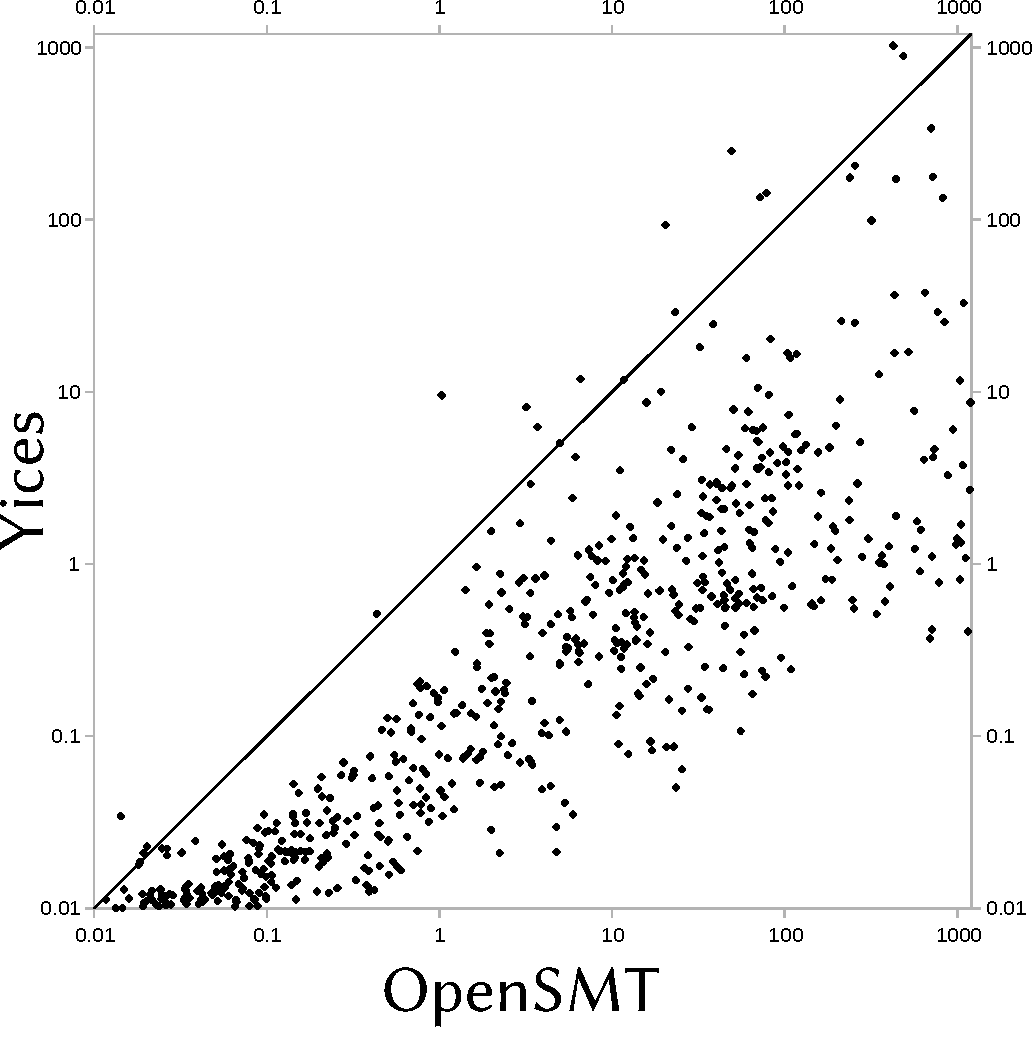
\includegraphics[width=0.49\linewidth]{comp_yices}
		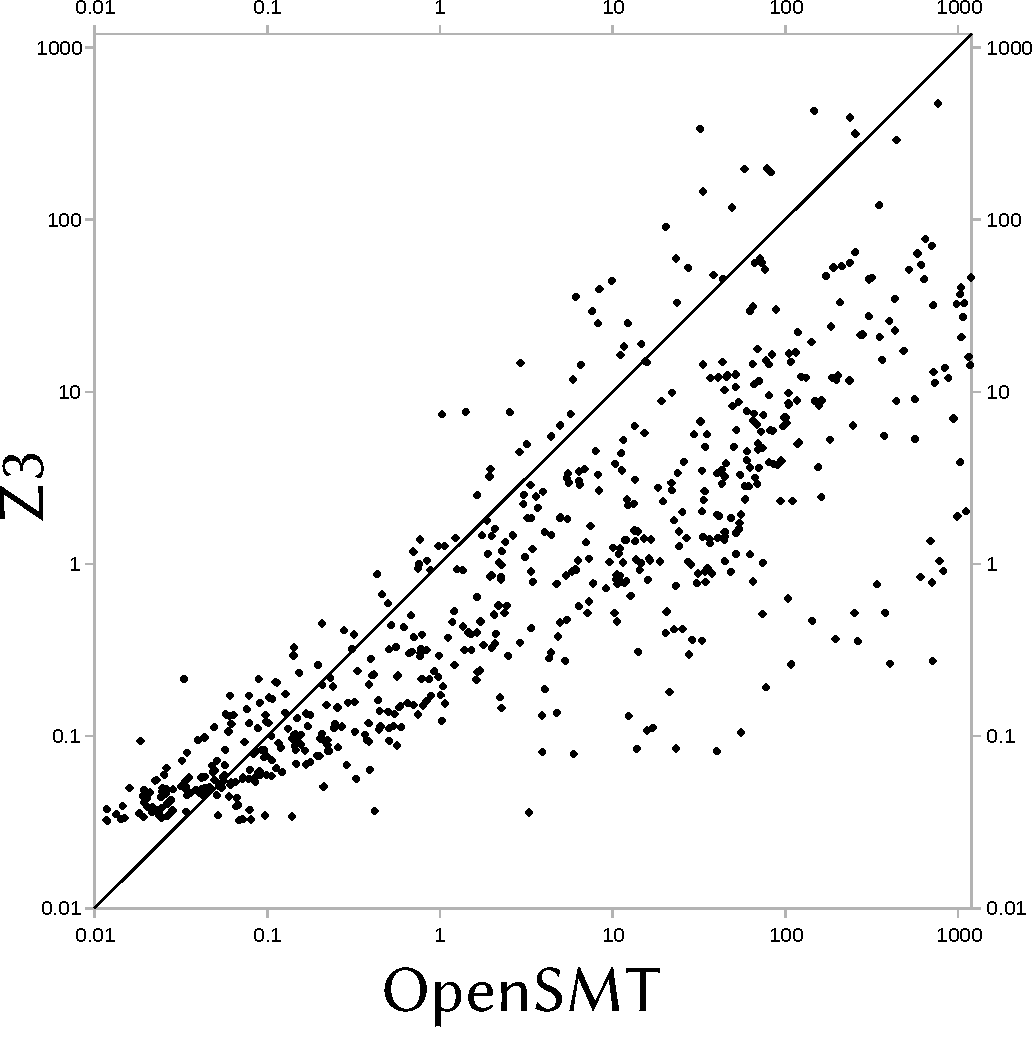
\includegraphics[width=0.49\linewidth]{comp_z3}\\
		\vspace{5px}
		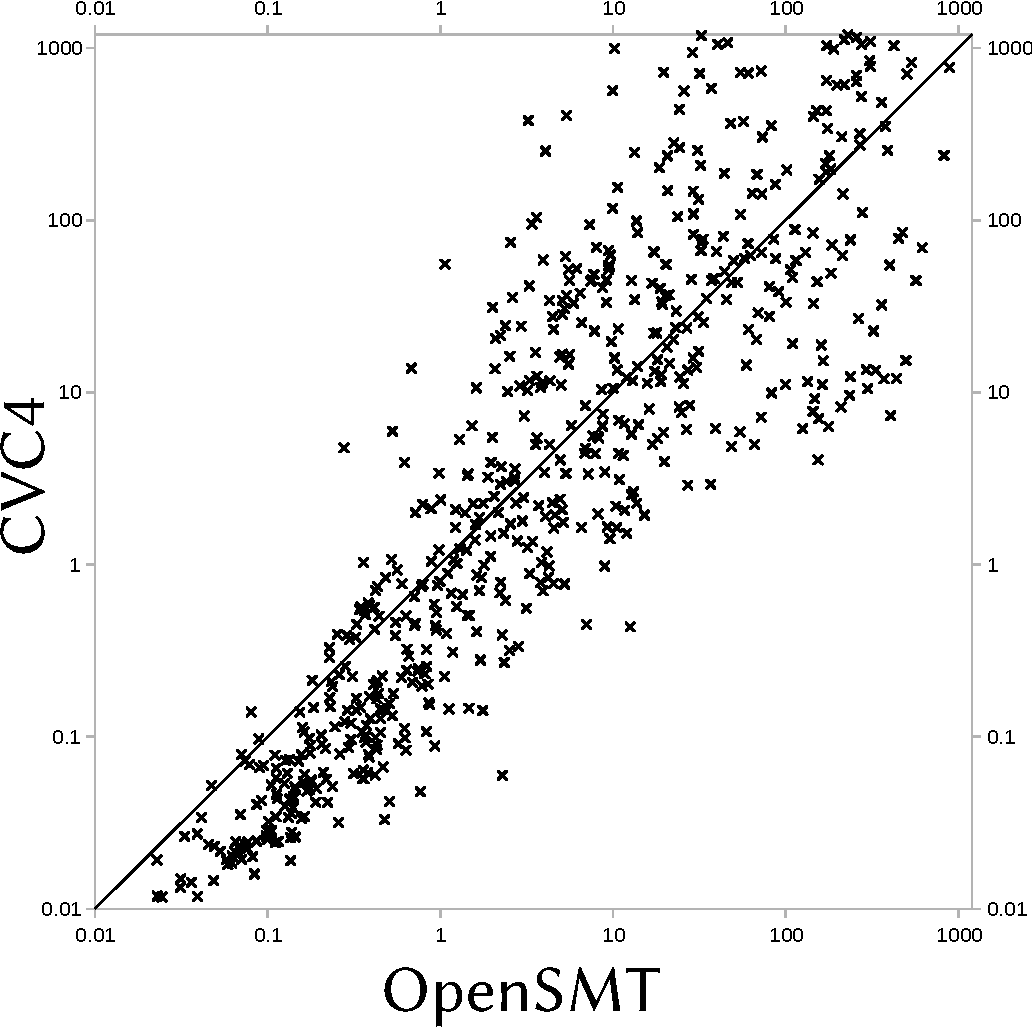
\includegraphics[width=0.49\linewidth]{comp_cvc}
		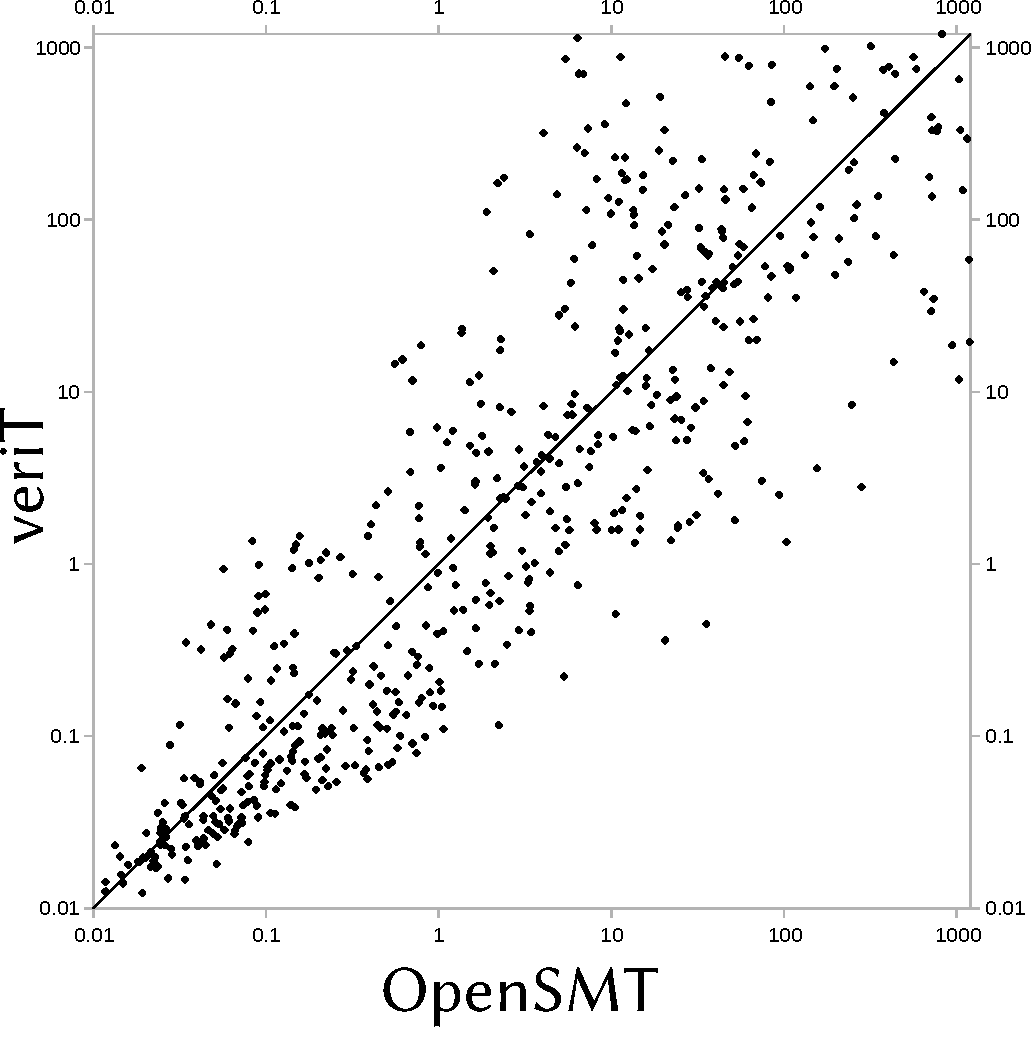
\includegraphics[width=0.49\linewidth]{comp_verit}\\
		\vspace{5px}
		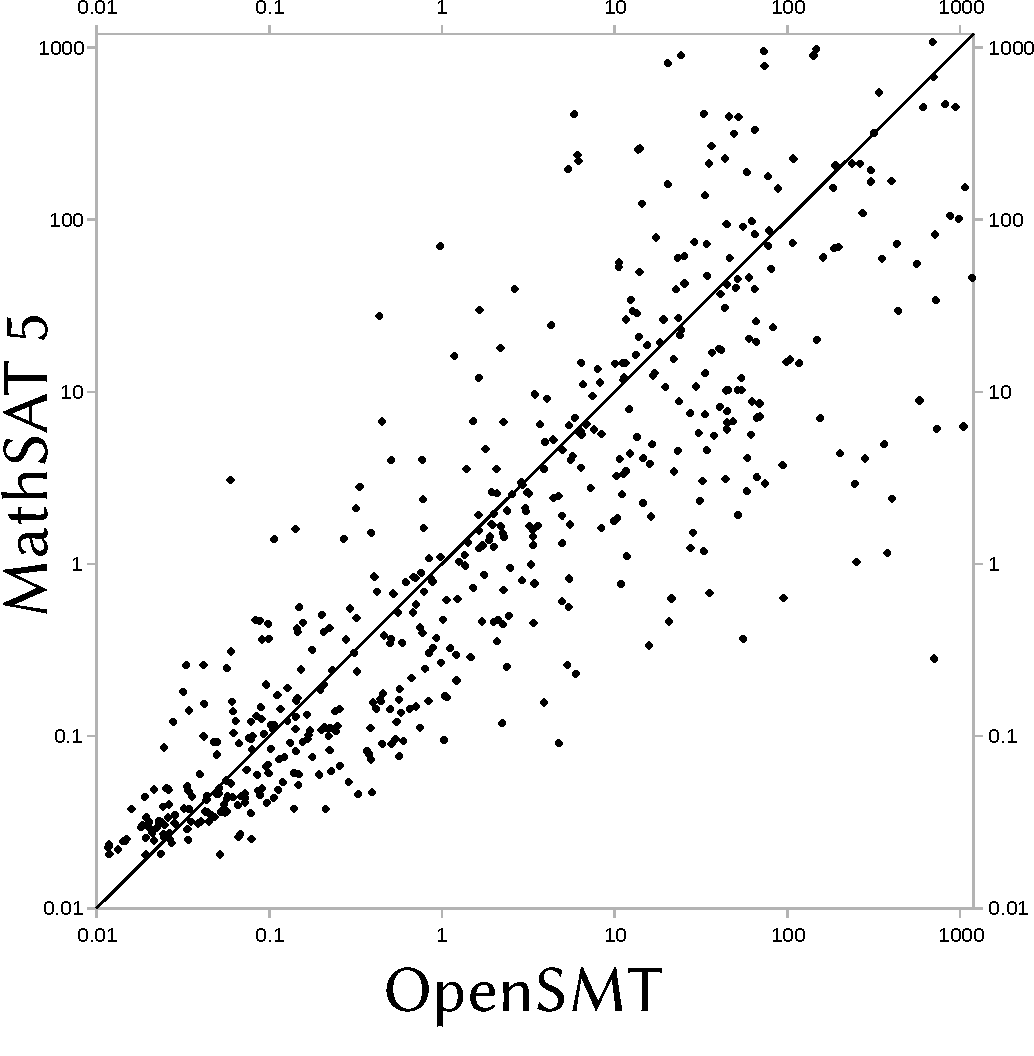
\includegraphics[width=0.49\linewidth]{comp_mathsat}
		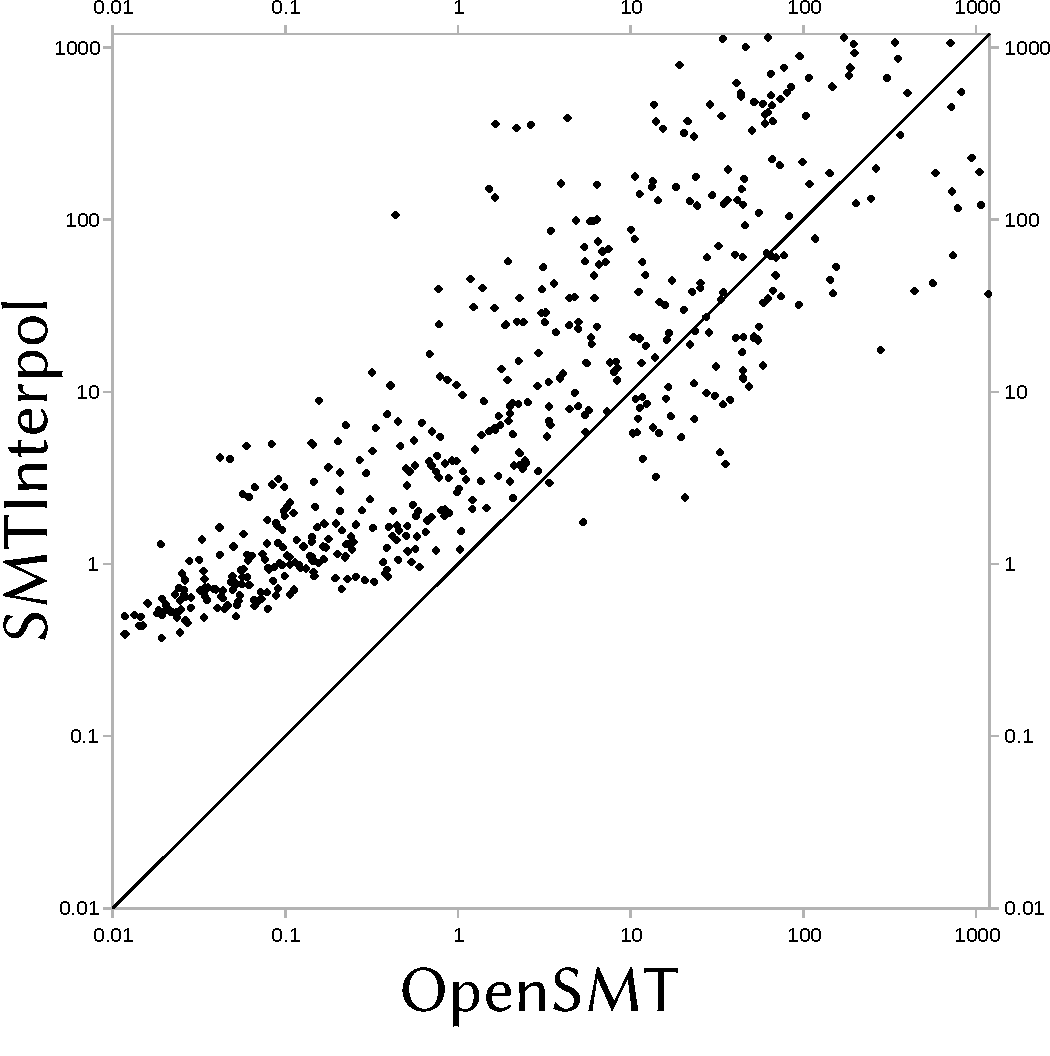
\includegraphics[width=0.49\linewidth]{comp_smti}
		\caption{Srovnání OpenSMT s~ostatními SMT řešiči na vyřešených testech}
\end{figure}

Jak vidíme, OpenSMT se zařadilo do průměru soutěžících --- v~letošním ročníku soutěže SMT-COMP by skončilo na čtvrtém místě. Nemůže se zatím rovnat s~nejlepšími řešiči Yices a~z3, které úspěšně vyřešily o~79, resp. o~62 testů více. Se všemi ostatními však má minimálně srovnatelné hodnocení. V~porovnání s~CVC4 jsme dosáhli takřka $97\,\%$ vyřešených testů a~byli jsme dokonce znatelně úspěšnější než řešiče veriT, SMTInterpol a~MathSAT.

Fakt, že náš řešič ve všech 661 vyřešených testech vrátil správné řešení, navíc můžeme brát jako relativně silný důkaz jeho korektnosti. Tyto výsledky tedy považujeme za úspěch jak frameworku OpenSMT, tak naší implementace řešiče diferenční logiky.


\chapter*{Závěr}
\addcontentsline{toc}{chapter}{Závěr}

V~rámci práce jsme pro OpenSMT vytvořili řešič diferenční logiky nad množinou celých čísel. Seznámili jsme se s~problémem STP, rozebrali jeho vlastnosti a~ukázali jeho transformaci na grafový problém. Zvážili jsme způsoby jeho řešení v~kontextu SMT řešičů a~analyzovali existující algoritmy navržené pro framework DPLL($T$). Popsali jsme metodu vyčerpávající propagace teorie a~její aplikaci pro diferenční logiku.

S~ohledem na tyto poznatky jsme pak implementovali samotný řešič teorie. Naším cílem přitom bylo vytvořit řešič, který bude dobře integrován se zbytkem frameworku a~dosáhne výkonu srovnatelného s~ostatními moderními SMT řešiči. Výsledek naší práce jsme s~těmito řešiči experimentálně srovnali a~ukázali jsme, že se nám podařilo daného cíle dosáhnout --- OpenSMT je srovnatelné či dokonce rychlejší než některé z~nejznámějších SMT řešičů současnosti. Nedosahuje zatím účinnosti těch naprosto nejrychlejších, na jejichž vývoji se soustavně podílí desítky dedikovaných výzkumníků. Věříme ale, že poskytuje dobrý základ, který už v~současné formě nabízí rozumnou alternativu k~současným řešičům a~jehož využitelnost bude růst s~budoucími zlepšeními. 

\subsection*{Možná budoucí rozšíření}

Hlavním úkolem v~nejbližší budoucnosti frameworku je rozšíření našeho řešiče o~podporu problémů nad doménou reálných čísel. S~využitím poznatků uvedených v~sekci~\ref{int_v_real} a~datových struktur již existujících v~OpenSMT máme za to, že by toto rozšíření nemělo být příliš náročné. Většina kódu existujícího v~implementaci celočíselné verze je totiž přenositelná mezi oběma variantami.

Dalším možným směrem budoucího vývoje je práce na zlepšení výkonnosti stávajícího řešiče. Jedním možným směrem této práce by byla analýza implementace použitého algoritmu. Jako příklad uveďme bližší průzkum možnosti použití vícevláknových procesů. Naše zběžné testování tyto přístupy sice zamítlo, ale podrobnější výzkum a~testování by mohly odhalit možnosti ke zrychlení řešiče. Druhou možností pro další výzkum v~tomto směru by pak mohlo být také využití jiných algoritmů v~rámci OpenSMT, ať už by se jednalo o~implementaci již existujících algoritmů, nebo o~vytvoření zcela nových postupů.


%%% Seznam použité literatury
%%% Seznam použité literatury (bibliografie)
%%%
%%% Pro vytváření bibliografie používáme bibTeX. Ten zpracovává
%%% citace v textu (např. makro \cite{...}) a vyhledává k nim literaturu
%%% v souboru literatura.bib.
%%%
%%% Příkaz \bibliographystyle určuje, jakým stylem budou citovány odkazy
%%% v textu. V závorce je název zvoleného souboru .bst. Styly plainnat
%%% a unsrt jsou standardní součástí latexových distribucí. Styl czplainnat
%%% je dodáván s touto šablonou a bibTeX ho hledá v aktuálním adresáři.

\bibliographystyle{czplainnat}    %% Autor (rok) s českými spojkami
% \bibliographystyle{plainnat}    %% Autor (rok) s anglickými spojkami
% \bibliographystyle{unsrt}       %% [číslo]

\renewcommand{\bibname}{Seznam použité literatury}

%%% Vytvoření seznamu literatury. Pozor, pokud jste necitovali ani jednu
%%% položku, seznam se automaticky vynechá.

\bibliography{literatura}

%%% Kdybyste chtěli bibliografii vytvářet ručně (bez bibTeXu), lze to udělat
%%% následovně. V takovém případě se řiďte normou ISO 690 a zvyklostmi v oboru.

% \begin{thebibliography}{99}
%
% \bibitem{lamport94}
%   {\sc Lamport,} Leslie.
%   \emph{\LaTeX: A Document Preparation System}.
%   2. vydání.
%   Massachusetts: Addison Wesley, 1994.
%   ISBN 0-201-52983-1.
%
% \end{thebibliography}


%%% Obrázky v bakalářské práci
%%% (pokud jich je malé množství, obvykle není třeba seznam uvádět)
%%% \listoffigures

%%% Tabulky v bakalářské práci (opět nemusí být nutné uvádět)
%%% U matematických prací může být lepší přemístit seznam tabulek na začátek práce.
%%% \listoftables

%%% Použité zkratky v bakalářské práci (opět nemusí být nutné uvádět)
%%% U matematických prací může být lepší přemístit seznam zkratek na začátek práce.
%%% \chapwithtoc{Seznam použitých zkratek}

%%% Přílohy k bakalářské práci, existují-li. Každá příloha musí být alespoň jednou
%%% odkazována z vlastního textu práce. Přílohy se číslují.
%%%
%%% Do tištěné verze se spíše hodí přílohy, které lze číst a prohlížet (dodatečné
%%% tabulky a grafy, různé textové doplňky, ukázky výstupů z počítačových programů,
%%% apod.). Do elektronické verze se hodí přílohy, které budou spíše používány
%%% v elektronické podobě než čteny (zdrojové kódy programů, datové soubory,
%%% interaktivní grafy apod.). Elektronické přílohy se nahrávají do SISu a lze
%%% je také do práce vložit na CD/DVD. Povolené formáty souborů specifikuje
%%% opatření rektora č. 72/2017.
\appendix
\chapter{Přílohy}

\section{První příloha}

\openright
\end{document}
